Initially, the raw data was distributed into multiple .csv files (one file per user, per time interval). The files were read and processed by the Python Pandas\footnote{\url{https://pandas.pydata.org}} tool. The library offers fast and flexible functionalities for data analysis. It utilises DataFrames which are fast and efficient 2D data structures, used to store tabular data. Using the Pandas \textit{read\_csv}\footnote{\url{https://pandas.pydata.org/pandas-docs/stable/reference/api/pandas.read_csv.html}} and \textit{concat}\footnote{\url{https://pandas.pydata.org/pandas-docs/stable/reference/api/pandas.concat.html}} methods, the files with identical time periods were transformed and concatenated to one collective DataFrame. 


\subsubsection{Missing Values}
The raw data contained several rows with empty cells. Section \ref{section:MissingValues} mentions substitution of missing data, thus preserving rows, which could otherwise contain important information. In doing so however, the existing patterns could be disrupted. In order to maintain the data's patterns, rows with missing values were removed. Using the Pandas' \textit{dropna}\footnote{\url{https://pandas.pydata.org/pandas-docs/stable/reference/api/pandas.DataFrame.dropna.html}} function (deletes rows with missing values), all rows containing empty cells were dropped. Of the original 8283 rows from the 1 hour time period files, only 3279 (39.59\%) rows were complete and remained. In the 3 hour files, only 6218 from 14091 (44.13\%) persisted.

\subsubsection{Normalisation}
The recorded values from the different smartphone sensors were spread over different number ranges. For example, whilst the values that describe the screen-on-time ranged between -20 and 2.0, the light sensor values could reach from 0 to over 60,000. As explained in \ref{section:Normalisation}, values with higher ranges can inadvertently outweigh smaller values. To be sure that the values are weighted the same, the sklearn \textit{StandardScaler}\footnote{\url{http://scikit-learn.org/stable/modules/generated/sklearn.preprocessing.StandardScaler.html}}(Z-score Normalization) was used to normalize the data. As mentioned in section \ref{section:Normalisation}, Z-score normalization is more robust to outliers, that could otherwise bias Min-Max Normalization. Therefore, Z-score Normalization was used instead of Min-Max Normalization.



% To be sure that the values are weighted the same, initially the sklearn \textit{MinMaxScaler}\footnote{\url{https://scikit-learn.org/stable/modules/generated/sklearn.preprocessing.MinMaxScaler.html}} (Min-Max Normalization) was used to map all the values into the common range, e.g. [0,1]. Most of the values in the dataset ranged between 0 and just over 100. The light sensor values were the exception, with its values reaching above 60,000. 

\subsubsection{Selection of columns (attributes)}

% Also - compressing 1-N columns
In order to only use meaningful data to receive significant results, it was important to remove columns that did not contain any predictive content. The TIME column was removed for this reason. Since the TIME column only showed the time and date when the data was recorded periodically (in fixed intervals), it was different for each row (per user) like an index. It could have however bias the results if left in. 

To reduce the number of dimensions (number of columns), columns that had recorded the same feature but at different time lags (e.g. ACC1-N), were compressed to one column. Each unique feature only required one column, and therefore reduced the number of columns to only 8 (instead of 32 in the 1h dataset or 48 in the 3h dataset).


\subsubsection{Chain shaped data}
\label{section:chainShapedData}
Initial visualisations of the dataset (with t-SNE dimensionality reduction) showed a chain formalisation of the data across various t-SNE parameters. This chain can be seen in figure \ref{figure:tsneChain} (light blue data points, almost swirl shaped). A similar accumulation of data points, though this time shaped as a line, can further also be seen in the PCA dimensionality reduced dataset (see figure \ref{figure:pcaChain}). 


\begin{figure*}[h]
  \centering
  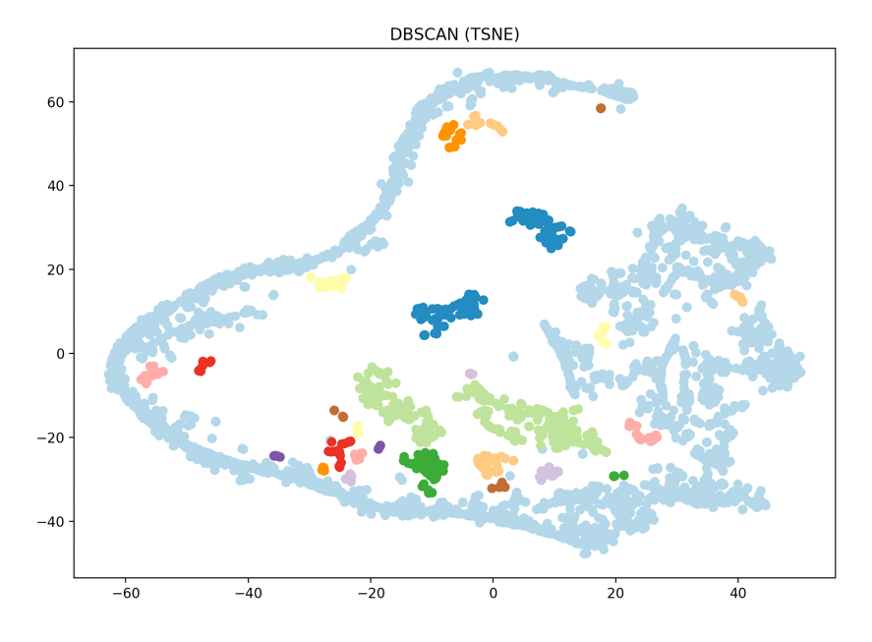
\includegraphics[width=0.7\textwidth]{./images/tsneChain.png}
  \caption{1h dataset, a chain of data points (light blue points) can be seen in the dataset.}
  \label{figure:tsneChain}
\end{figure*}


\begin{figure*}[h]
  \centering
  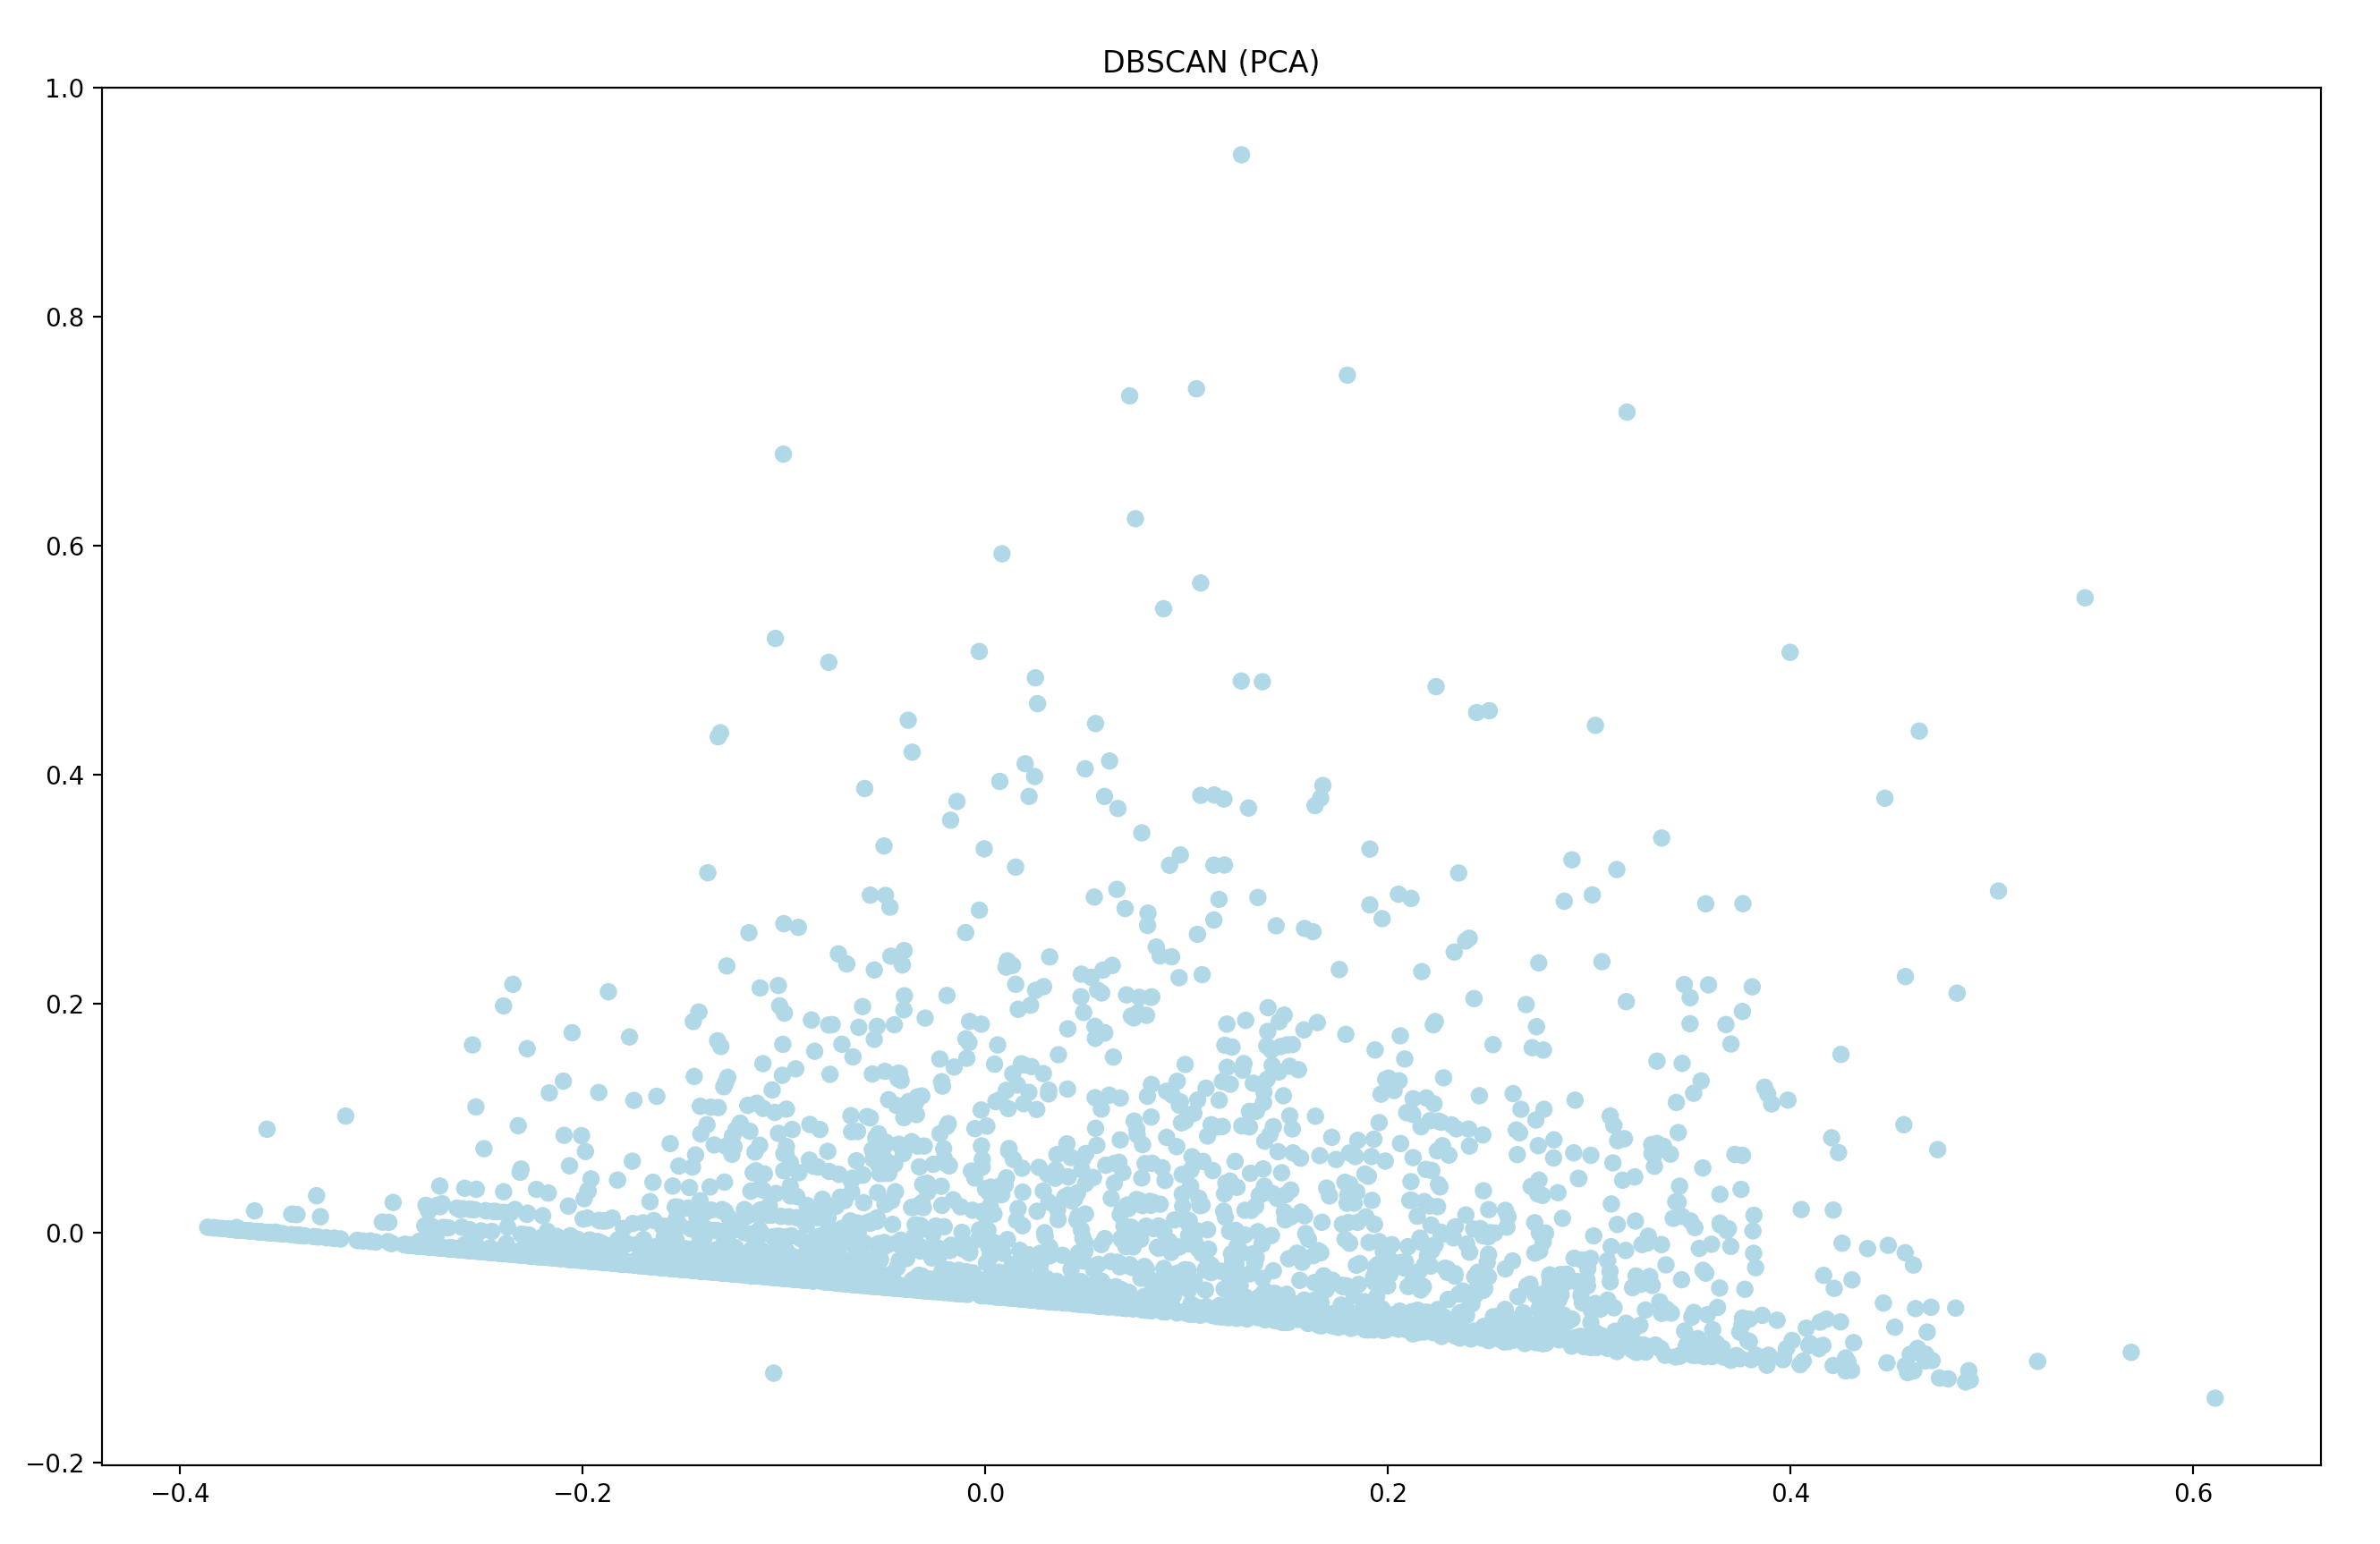
\includegraphics[width=0.7\textwidth]{./images/pcaChain.png}
  \caption{There is a collection of points along a line. This same collection can also be visualised as a chain in the t-SNE dataset in figure \ref{figure:tsneChain}.}
  \label{figure:pcaChain}
\end{figure*}

% An initial idea, was that this chain was the result of the utilised t-SNE parameters. However, even with changing the t-SNE perplexity, learning rate and number of iterations parameters, the chain persisted in some form. 
% The initial though, as to where these data points originated from or why they resulted in a chain, 
An initial thought, was that the chain was a consequence of dependencies within the data or columns. For example, the three APP columns indicate the percentage of time in a lag-interval a certain type of app was used. Therefore, if say a communication app was used 100\% of this time, the APP\_COM cell for this time would be 1. Using this app for 100\% of the time would mean, that the values in the other APP columns for this time would have to be 0 (0\%), since they would not have been able to be used. To test this theory, the APP columns were removed from the dataset and the 2D scatter plot was recalculated. The chain however was still visible. Step by step each column was removed, to see if it was the cause of the chain. The chain did not disappear though, which indicated, that the problem was not due to the columns, but rather the rows.  The chain also became less dense and less visible when reducing the number of inserted .csv files (lower number of records). This supported the notion, that the rows could be the cause.

% The chain was less visible when reducing the number of inserted .csv files (lower number of records) to 10 (see figure \ref{figure:tsne10Files}). When the number of features were reduced to only AUDIO and ACC (two columns), the chain was once again visible (see figure \ref{figure:tsne10Files2Features}). The presumption was that when there were less data points and more features (e.g. 10 files but using all the features), there were enough different data points and the chain was less dense, making it less noticeable. When there were less data points but with less features (e.g. 10 files but using only 2 features), or when there were many data points even with multiple features (e.g. all data files and all the features), there were more rows with very similar or equal values and the chain appears more dense and prevalent.

% \begin{figure*}[h]
%   \centering
%   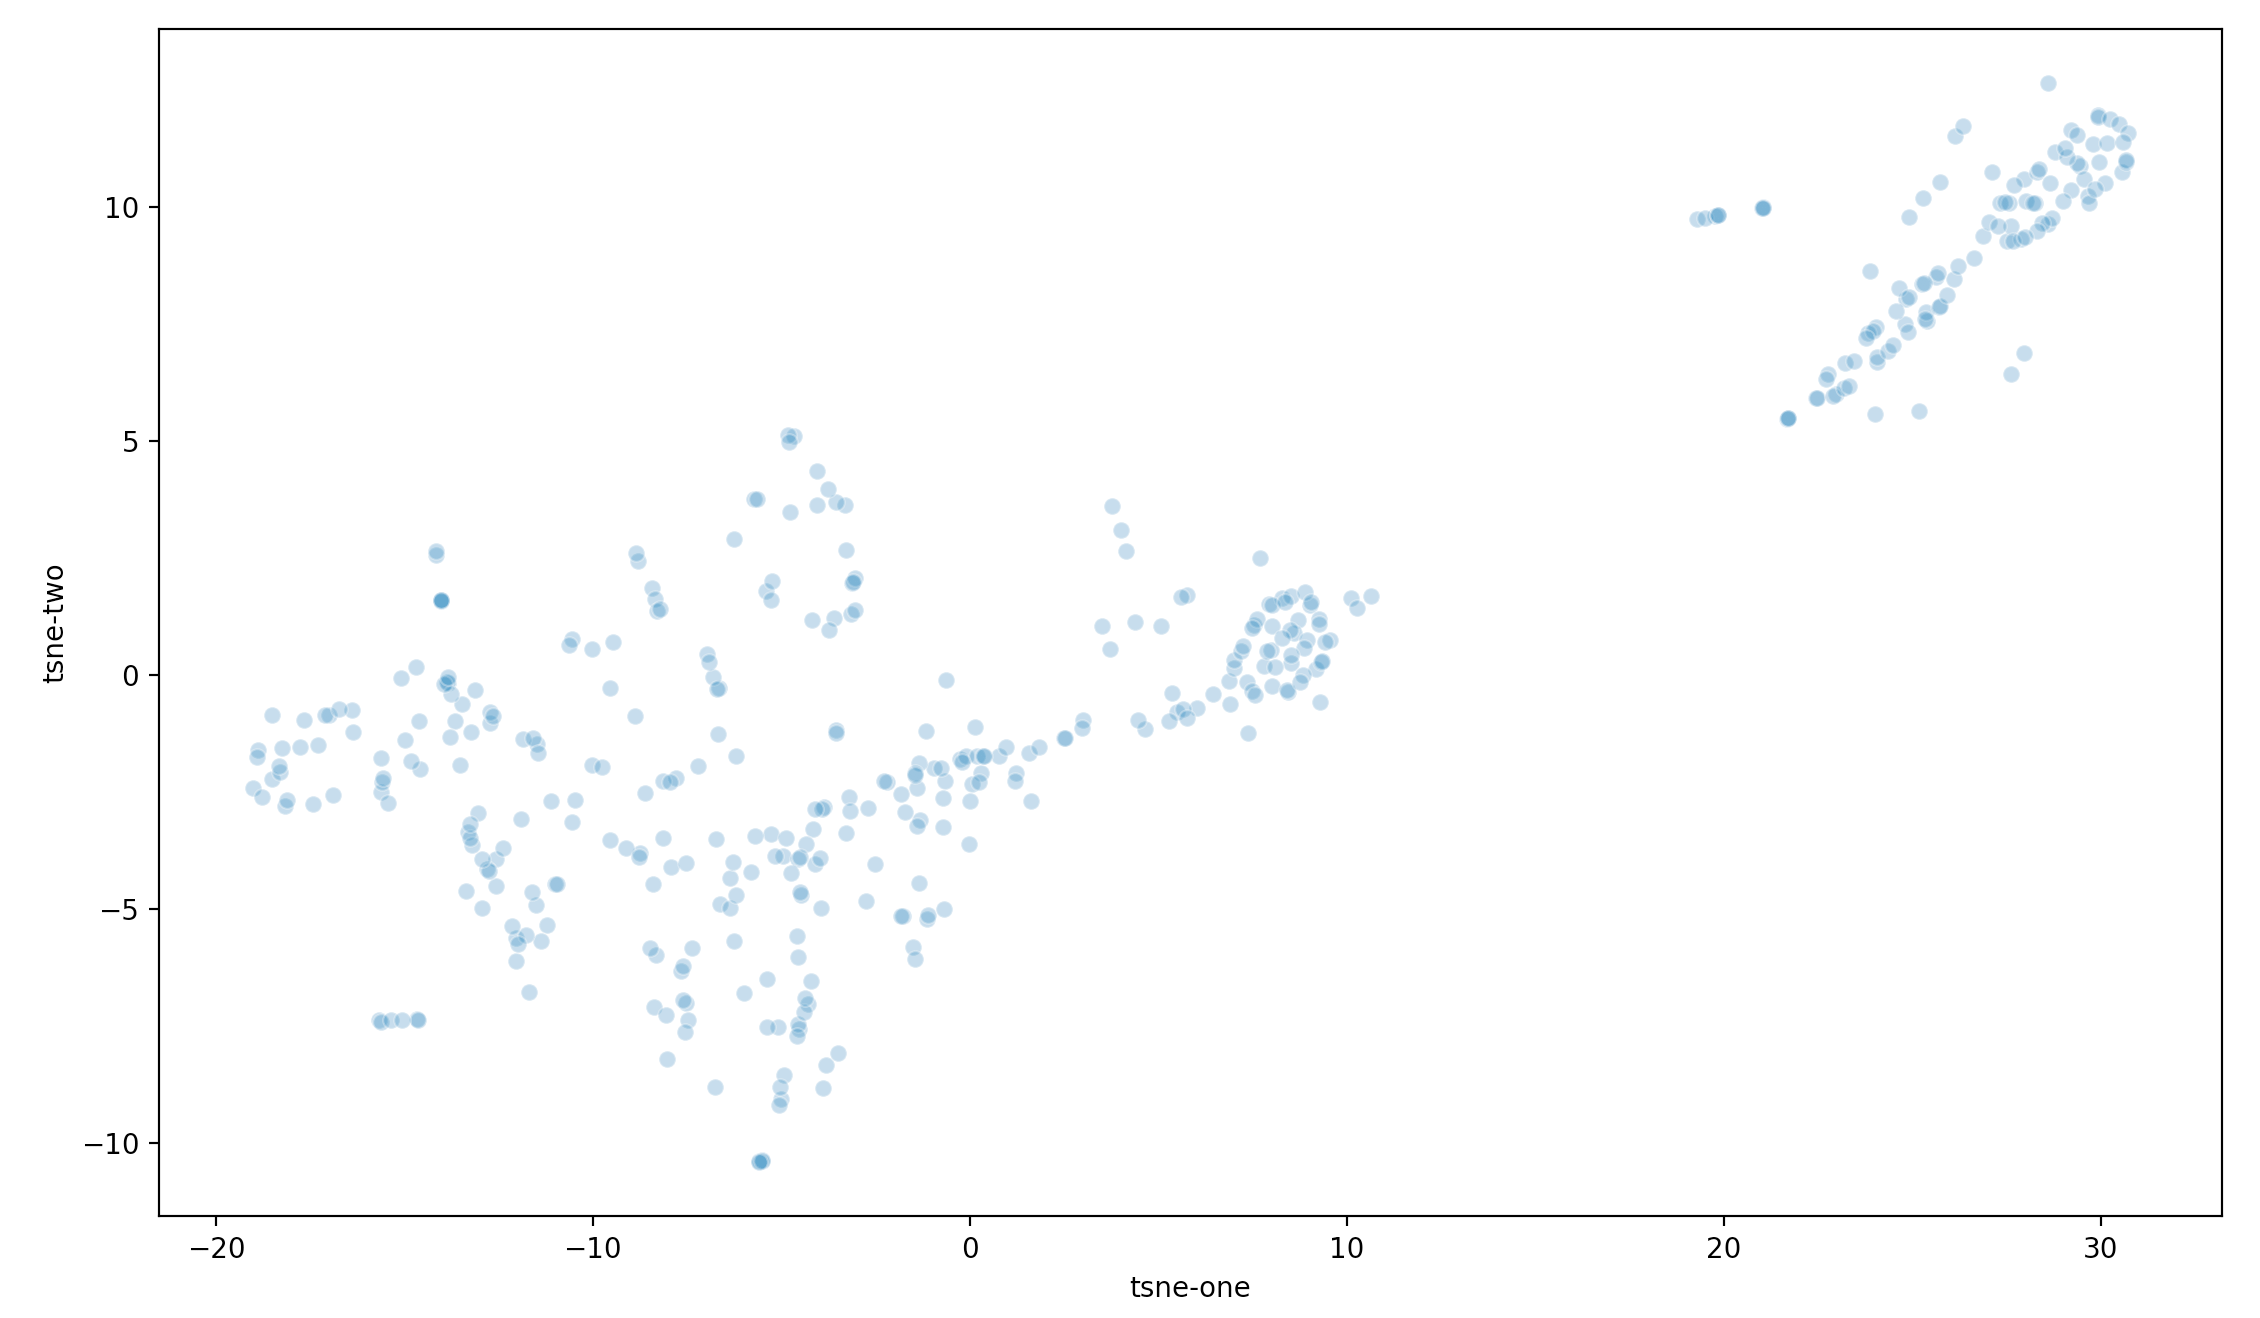
\includegraphics[width=0.5\textwidth]{./images/tsne10Files.png}
%   \caption{t-SNE calculated with only 10 data files and all features. The chain is as visible.}
%   \label{figure:tsne10Files}
% \end{figure*}

% \begin{figure*}[h]
%   \centering
%   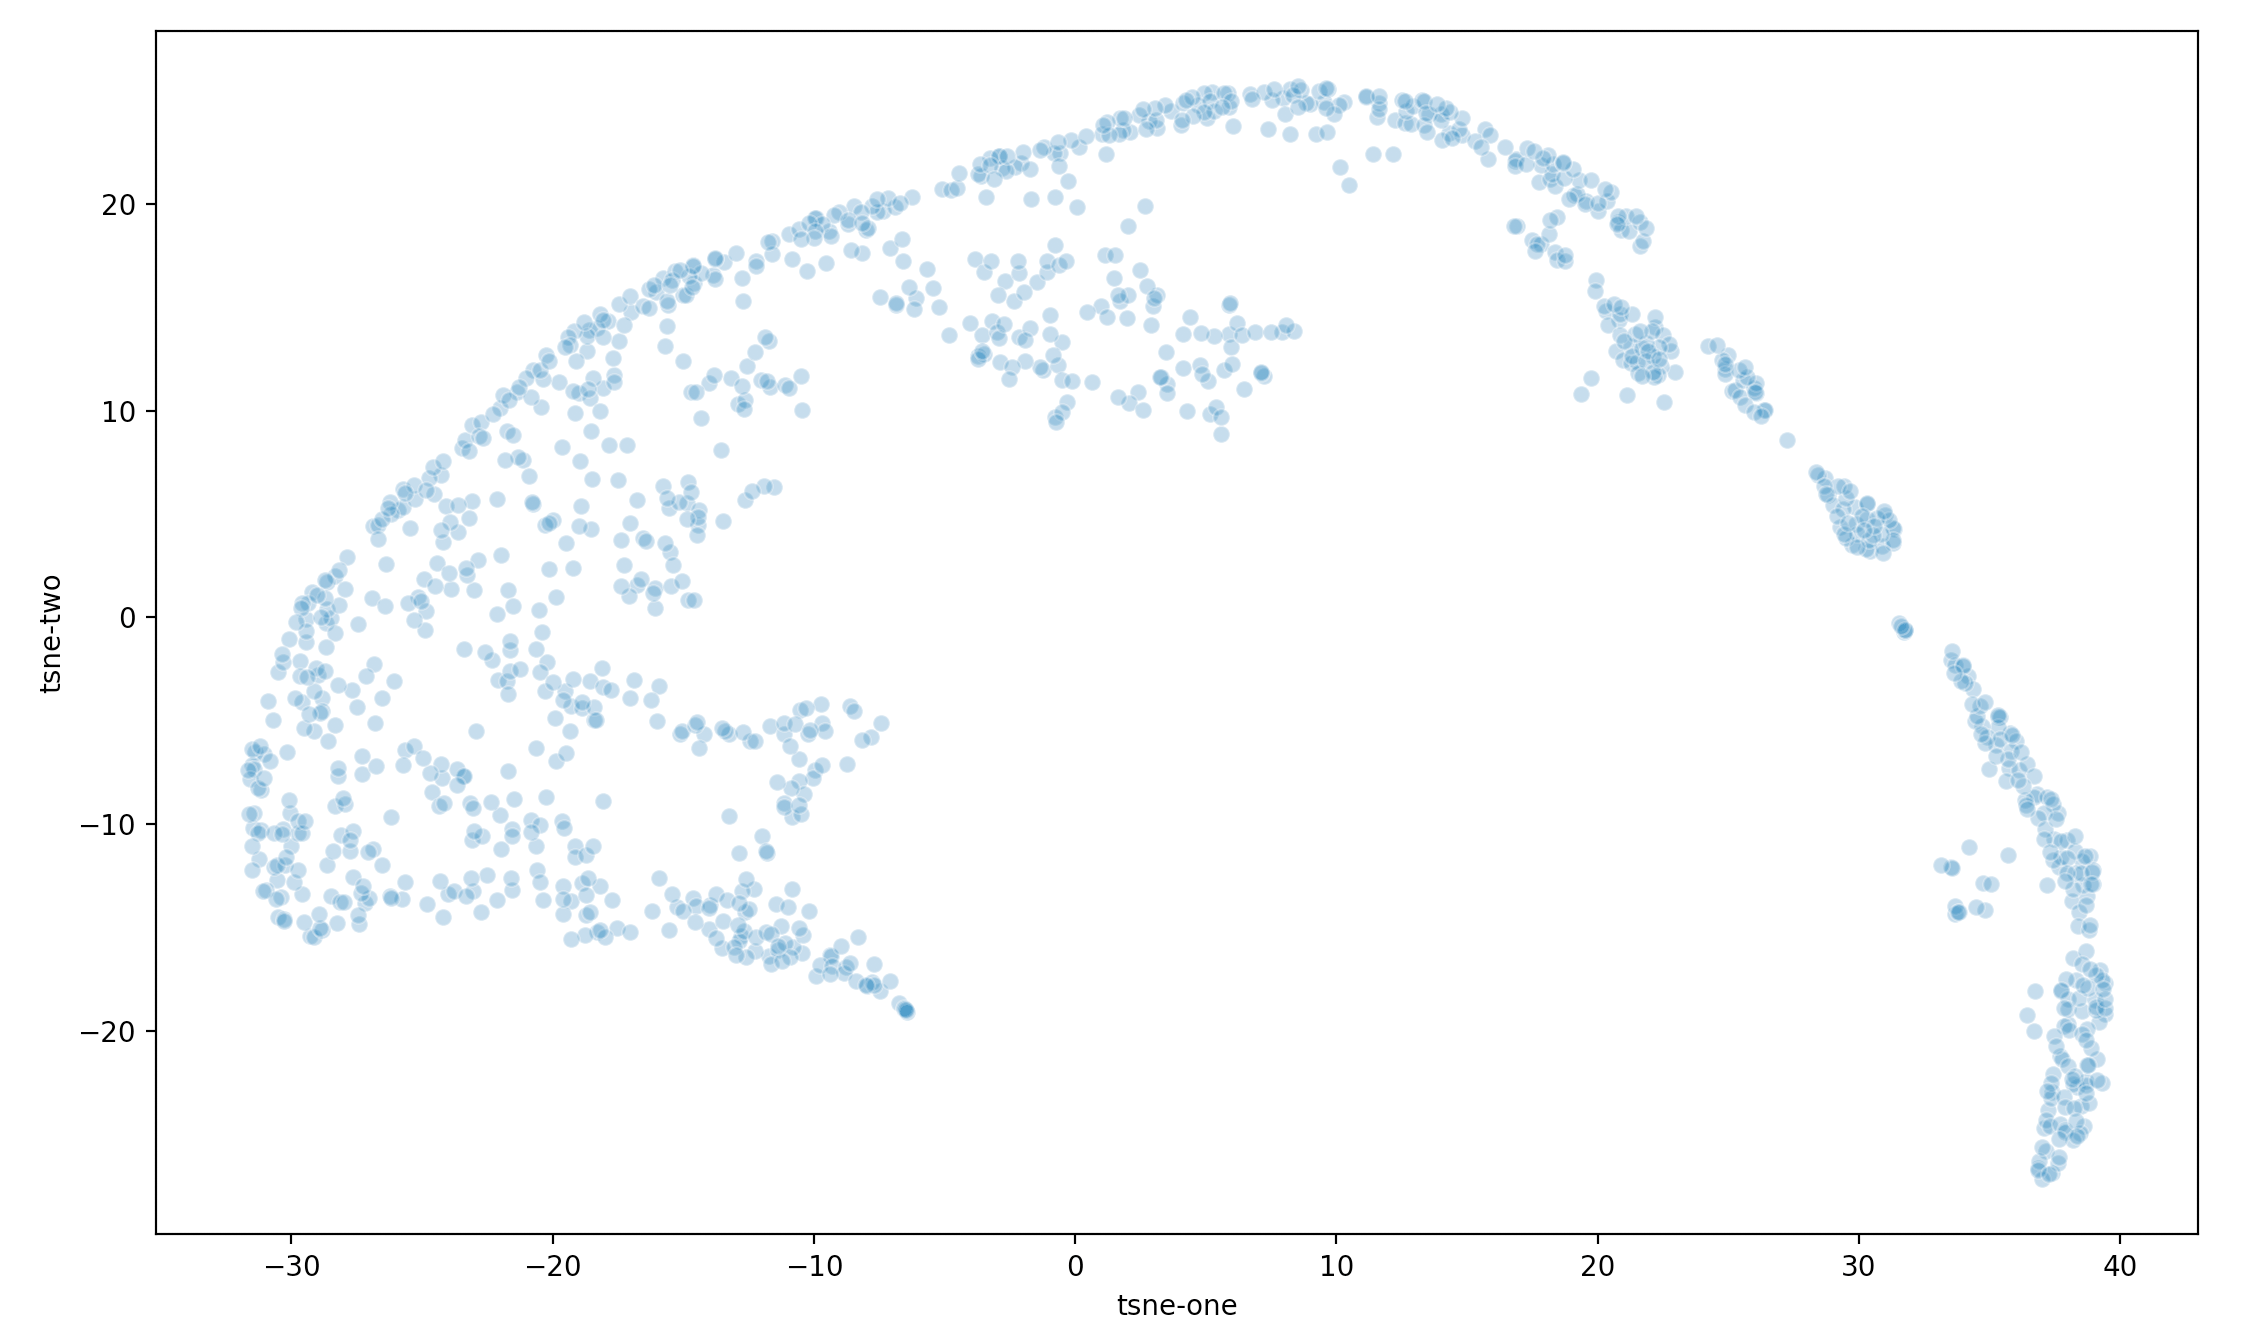
\includegraphics[width=0.5\textwidth]{./images/tsne10Files2Features.png}
%   \caption{t-SNE calculated with 10 data files and only 2 features. The chain is visible.}
%   \label{figure:tsne10Files2Features}
% \end{figure*}



% \begin{figure}[H]
%   \centering
%   \begin{subfigure}{.475\textwidth}
%     \centering
%     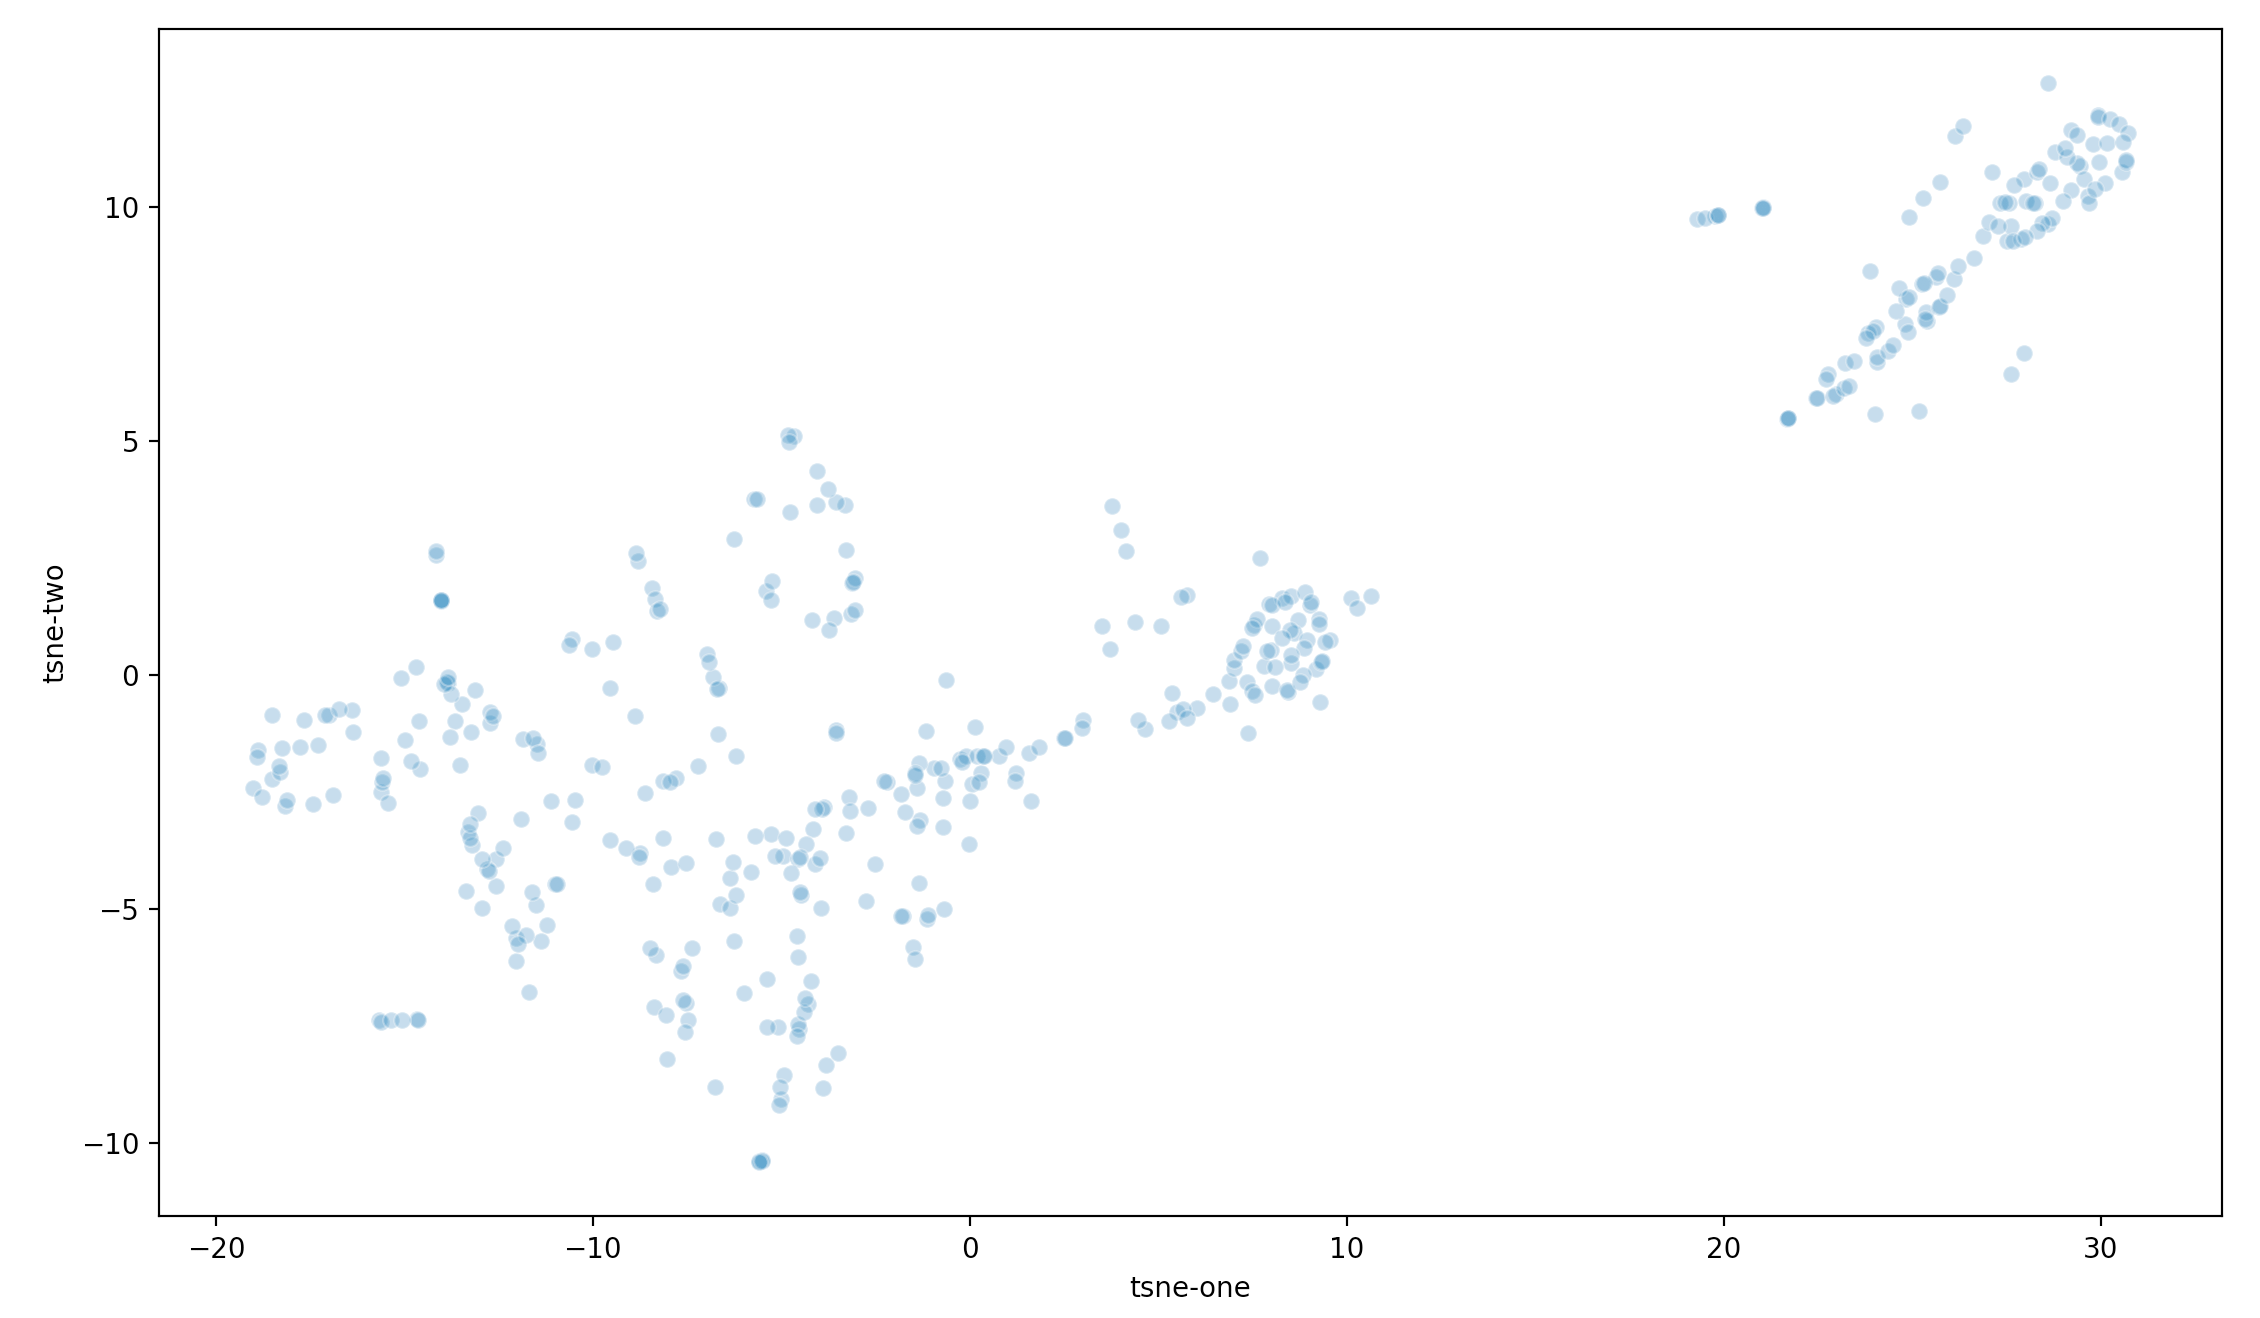
\includegraphics[width=1\textwidth]{./images/tsne10Files.png}
%     \caption{t-SNE calculated with only 10 data files and all features. The chain is not as visible.}
%     \label{figure:tsne10Files}
%   \end{subfigure}%
%   \hfill
%   \begin{subfigure}{.475\textwidth}
%     \centering
%     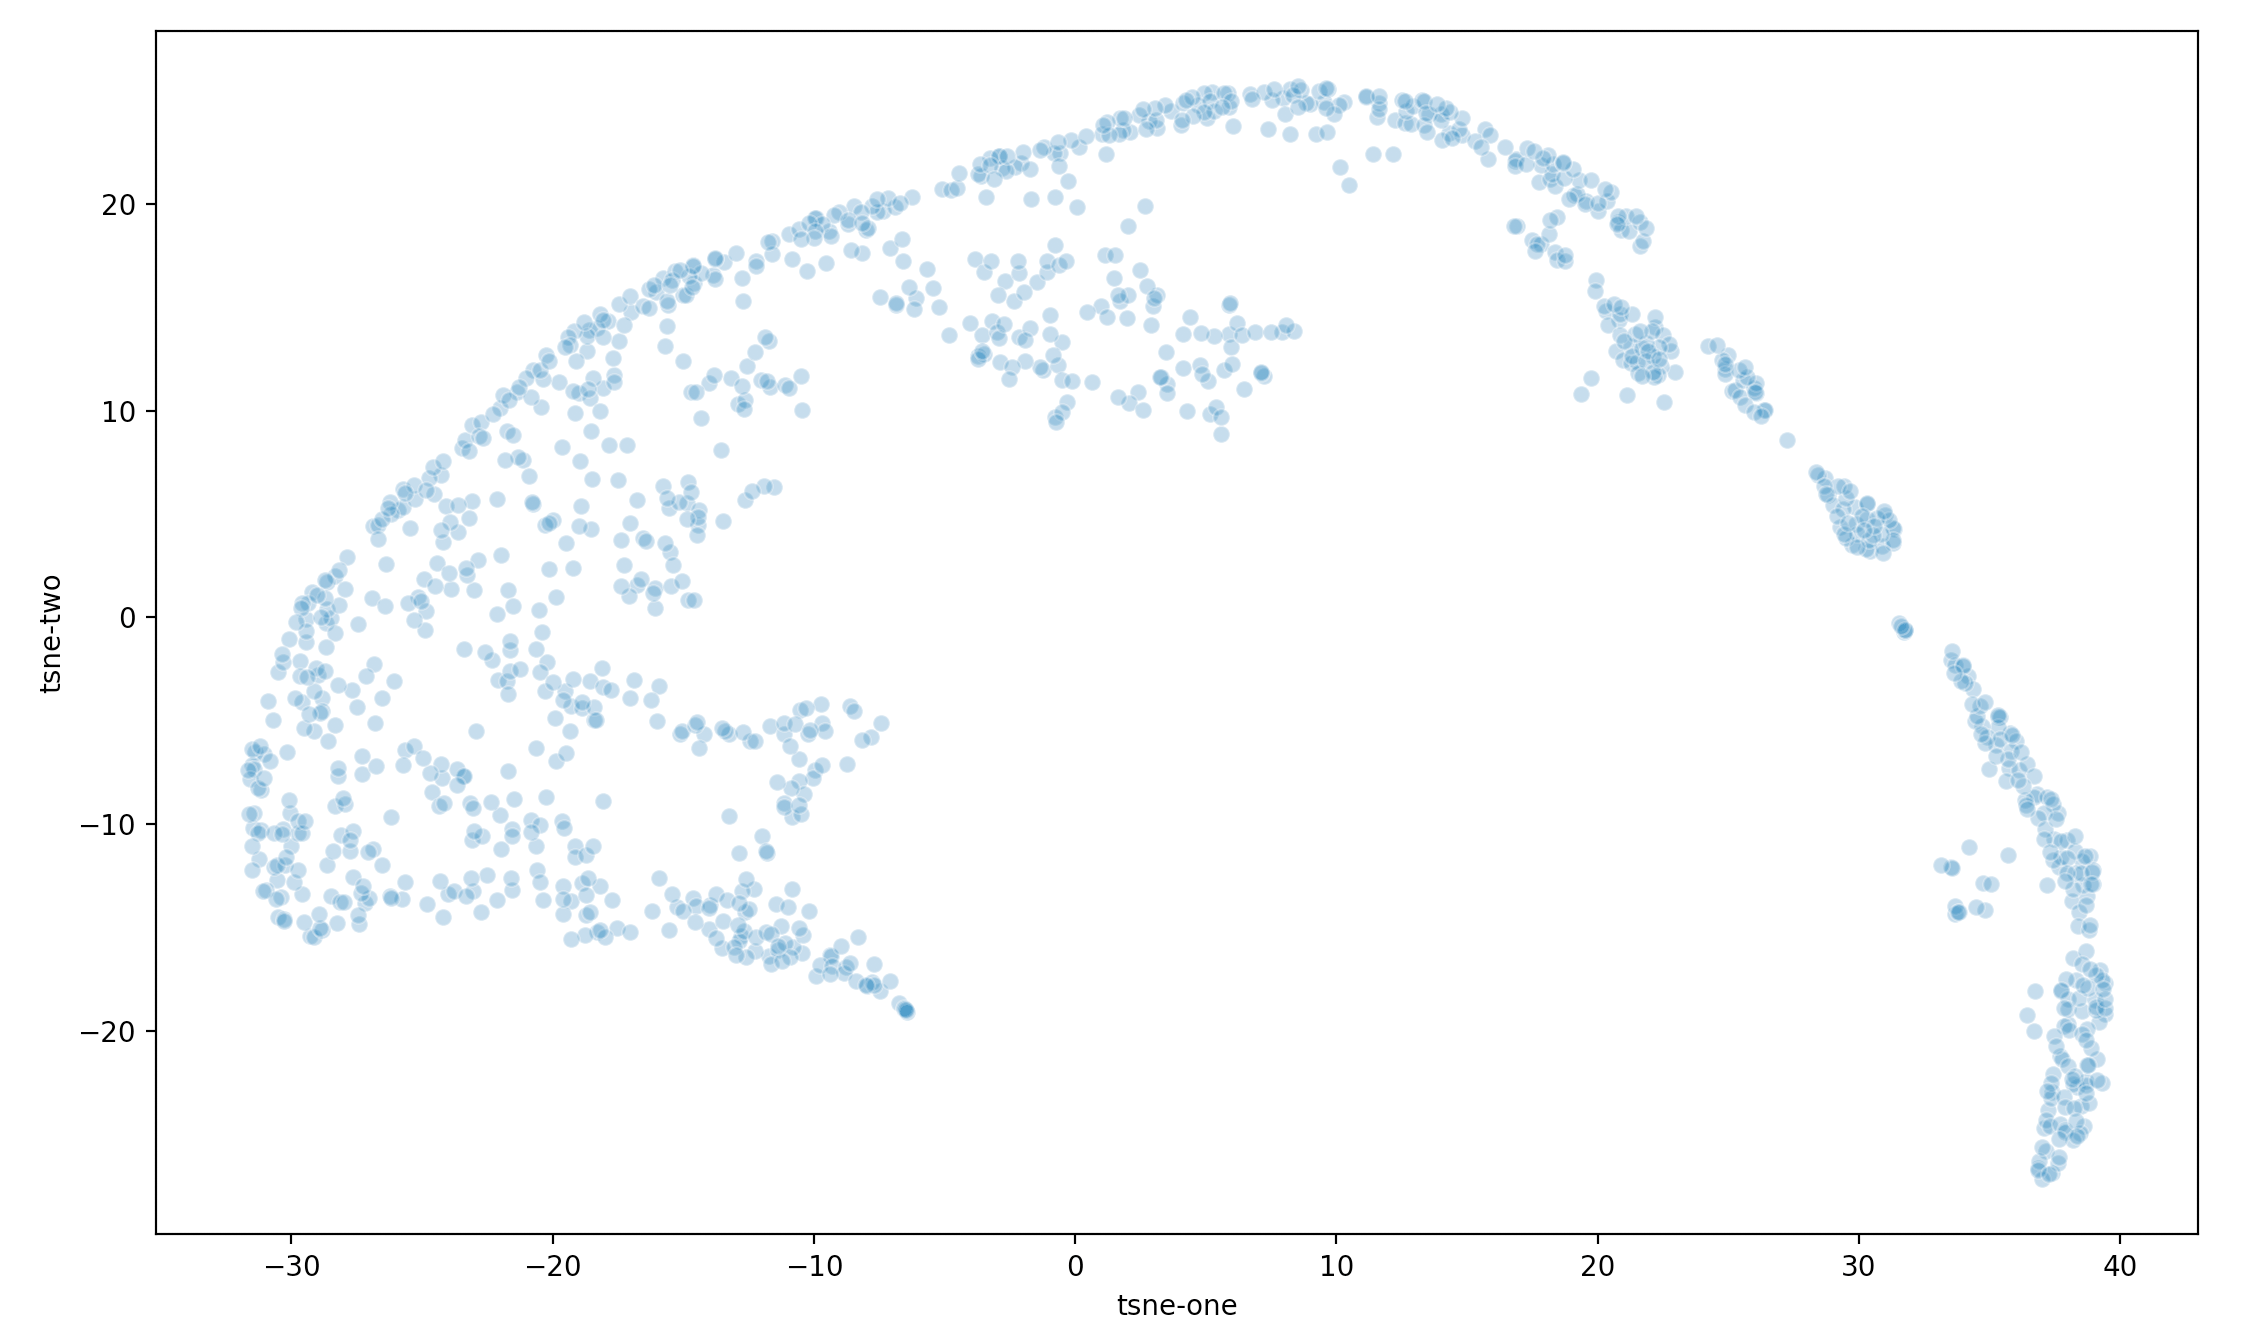
\includegraphics[width=1\textwidth]{./images/tsne10Files2Features.png}
%     \caption{t-SNE calculated with 10 data files and only 2 features. The chain is visible.}
%     \label{figure:tsne10Files2Features}
%   \end{subfigure}
% 	\caption{}
%   % \label{}
% \end{figure}

The next theory, was that points from a same test subject were similar and might be causing the chain. To see which data points were contained in the chain, the row index number was added as a label to each data point in the scatter plot. Furthermore, each test user data file was assigned a different random colour, so that in the plot, it was visible which data points belonged to the same user. The resulting scatter plot is visualised in figure \ref{figure:tsneTestSubjectsColor}. From this plot it can be seen, that several data points from the same test subject cluster together in the chain, indicating similarity. There are however points from each user in different locations of the chart, not only in the chain. This implied, that the chain was not being caused by the subjects. 

The ensuing step, was to use the data point indices to look for similarities in the values. It was evident that multiple rows shared a lot of the same feature values. Rows not in the chain however, had different values. Looking at the same rows in the unclean dataset (after concatenation of the .csv data files and removal of rows with missing values), rows found in the chain had several columns all with the value 0. Further inspection showed, that when the SCRN value was 0, LIGHT, NOTIF and the APP columns where also 0. When a smartphone screen is off, the apps are not being used, which explains why the APP columns were mostly 0. The NOTIF values were often 0, presumably because the user was not constantly receiving notifications. The environment light was also often 0 when SCRN was 0, maybe because it was in a pocket or bag. To test whether these rows were causing the chain to occur, rows with less than 50\% of values that weren't 0 were removed. As can be seen in figure \ref{figure:tsneAfterChainRemoved(50Percent)}, the chain is much less prevalent. The colours belonging to the test users are also more distributed. Naturally, this reduced the total number of rows left. As an example, the average number of rows left for the 1h data files, depending on the time length, was 1654 from initial 8283 (19.97\%). In the 3h dataset, only an average of 3976.5 from 14091 rows remained (28.22\%).


% 8283 .... 100%
% 1654...x

% 14091...100%
% 3976.5 ....x


\begin{figure*}[h]
  \centering
  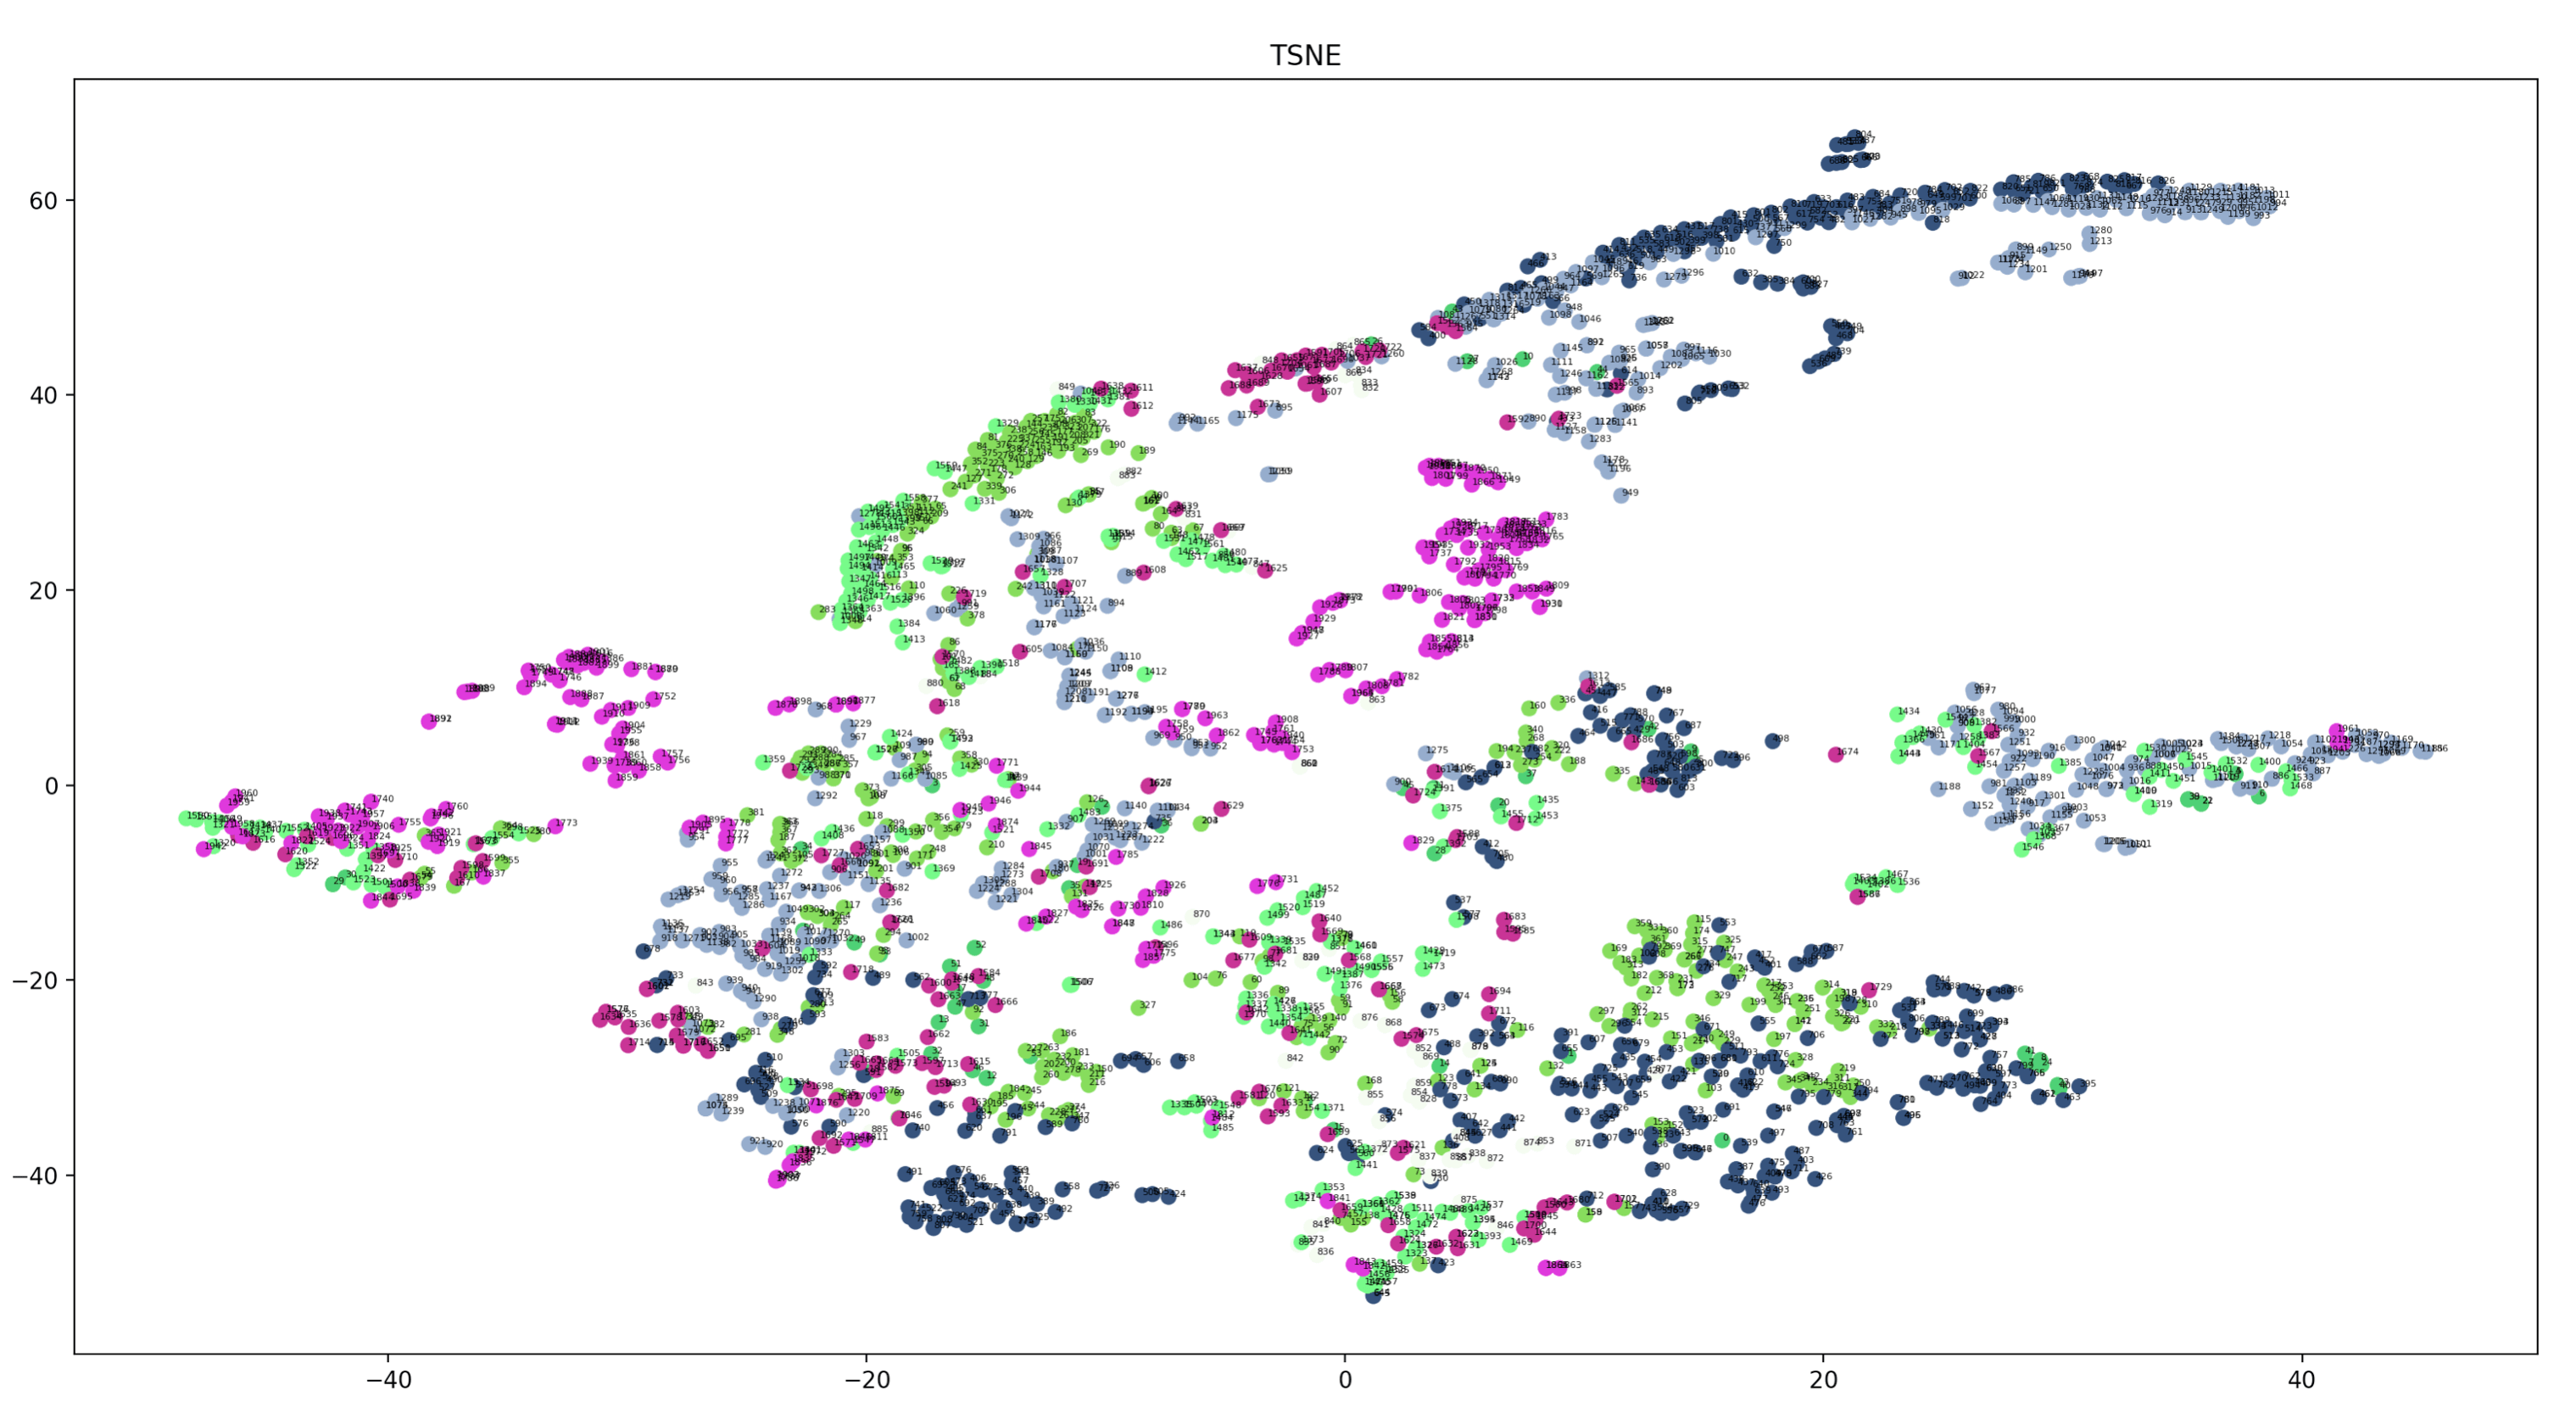
\includegraphics[width=0.9\textwidth]{./images/tsneTestSubjectsColor.png}
  \caption{t-SNE result in a scatter plot, each colour indicates one test subject. The test subjects have clustered together slightly in the chain.}
  \label{figure:tsneTestSubjectsColor}
\end{figure*}

\begin{figure*}[h]
  \centering
  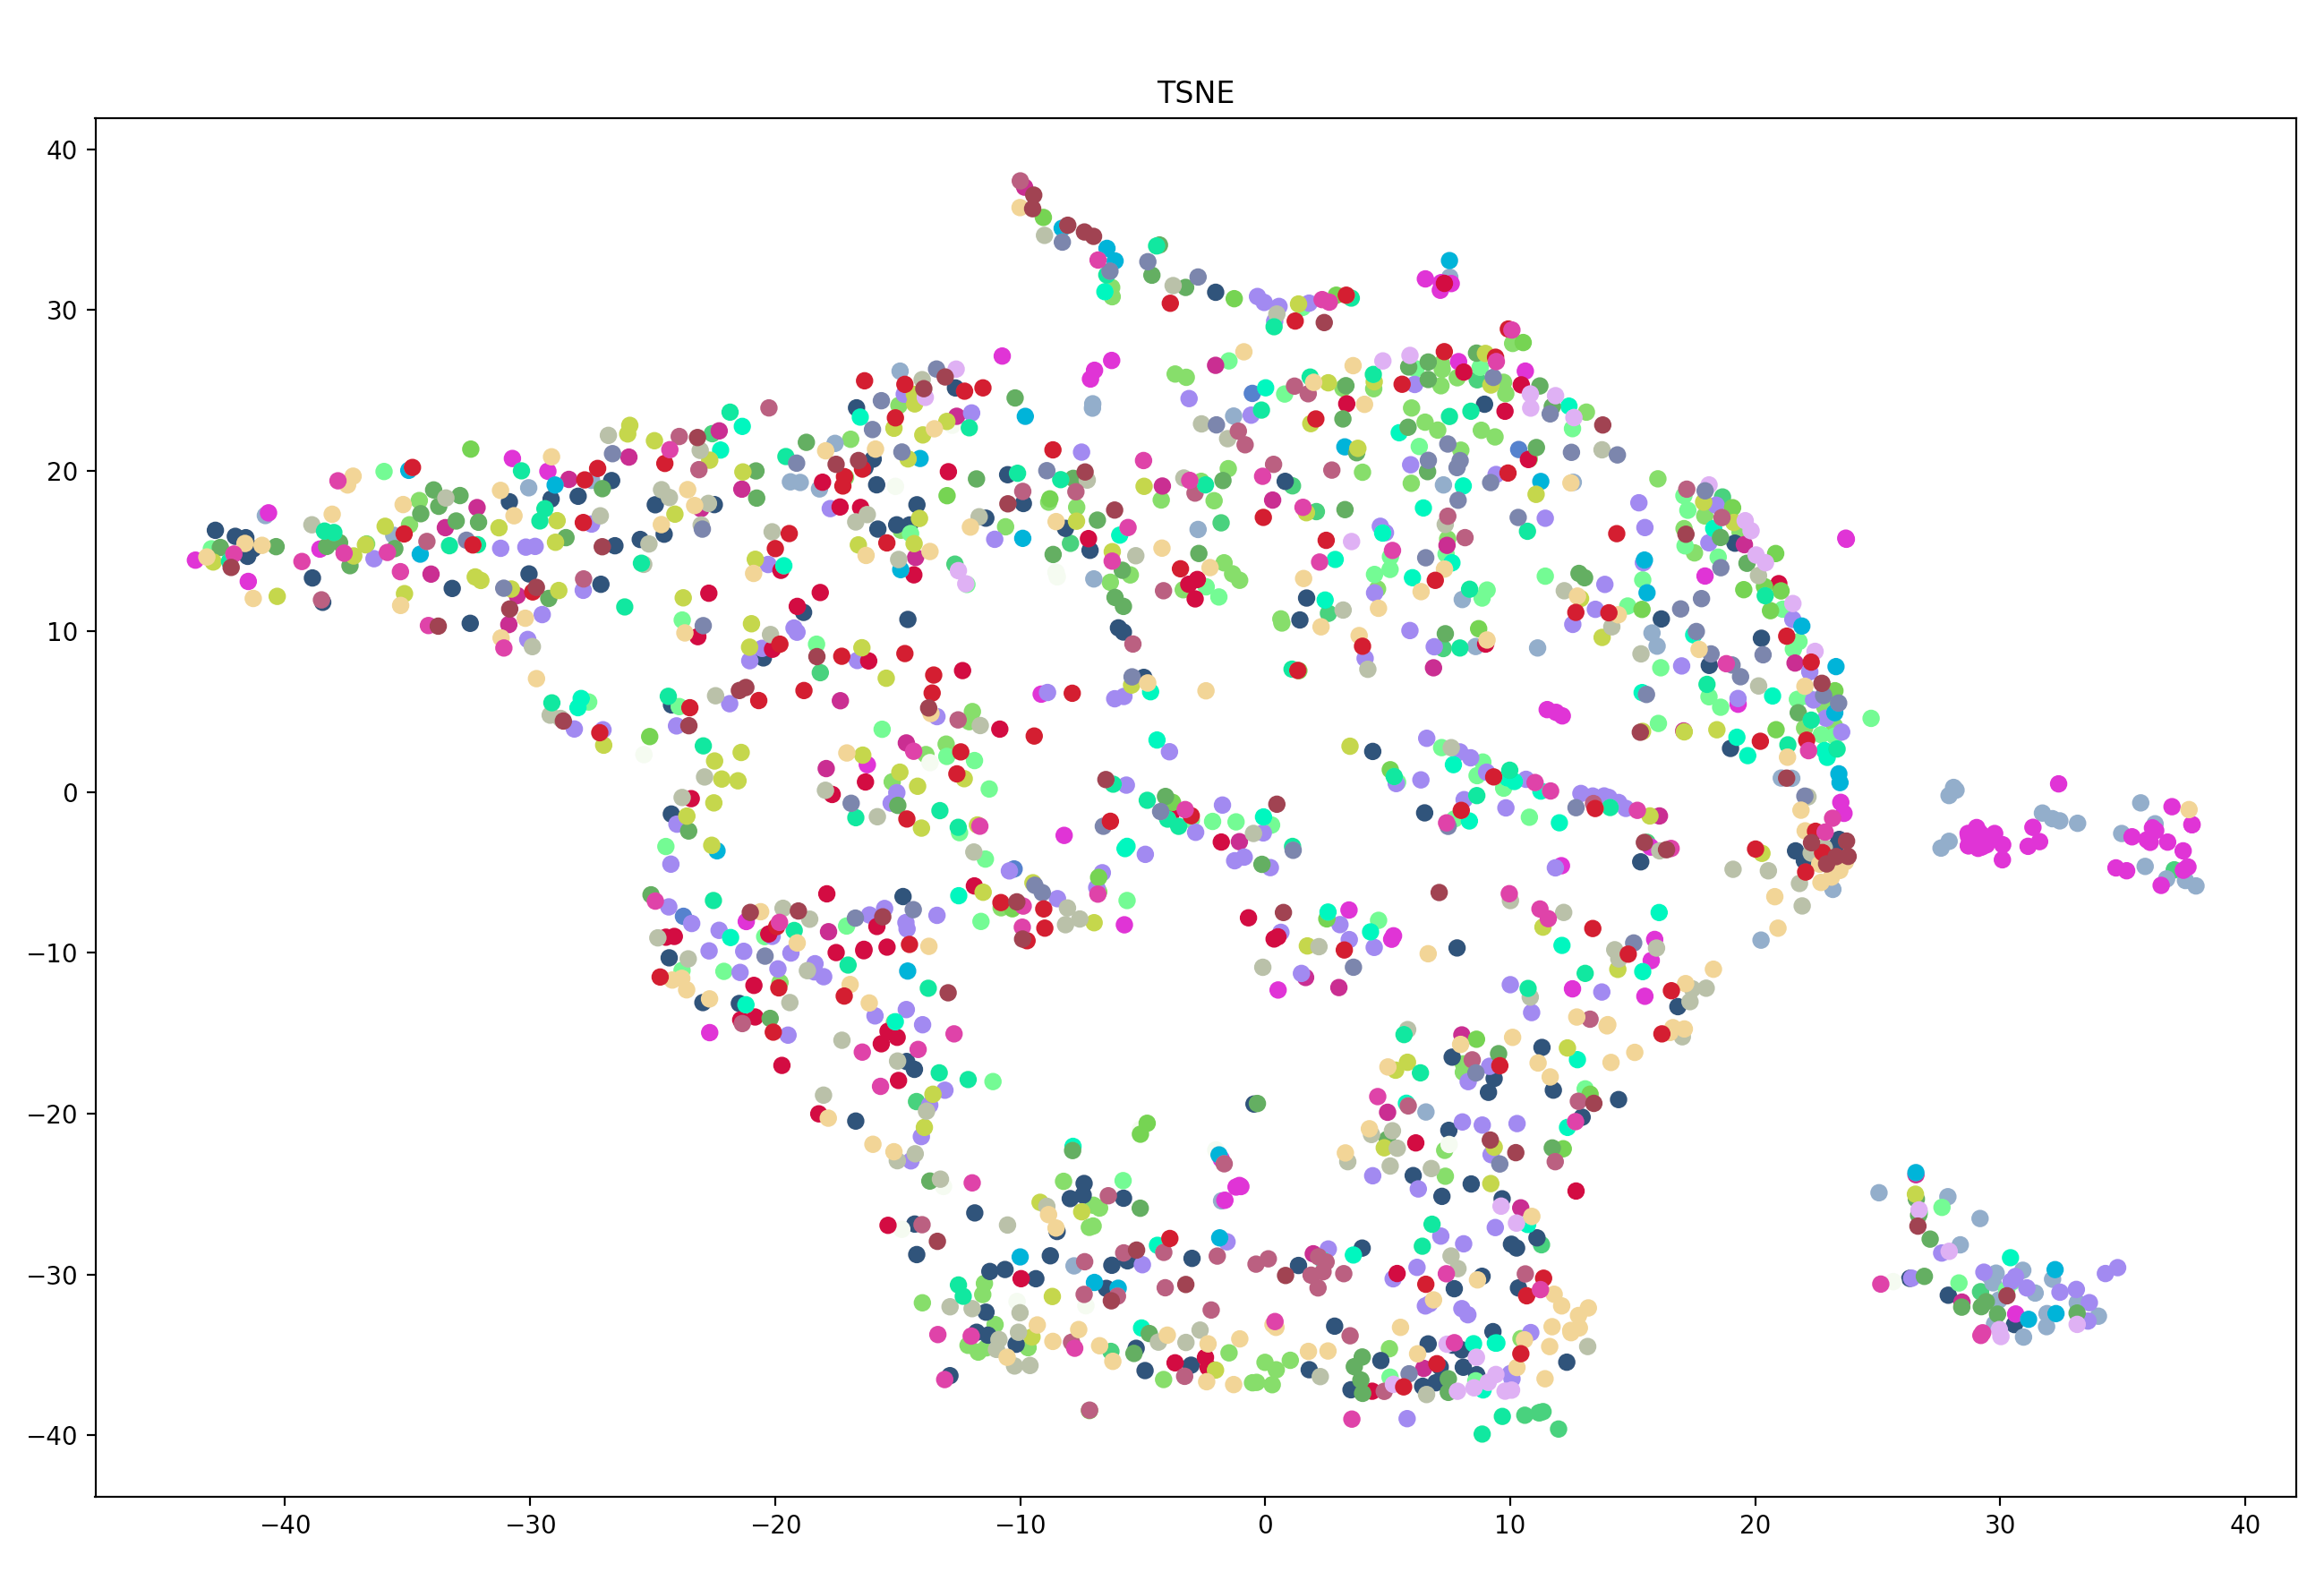
\includegraphics[width=0.9\textwidth]{./images/tsneAfterChainRemoved(50Percent).png}
  \caption{t-SNE calculated after the removal of rows with less than 50\% of values that weren't 0. The chain is less visible and less dominant.}
  \label{figure:tsneAfterChainRemoved(50Percent)}
\end{figure*}

% \begin{figure*}[h]
%   \centering
%   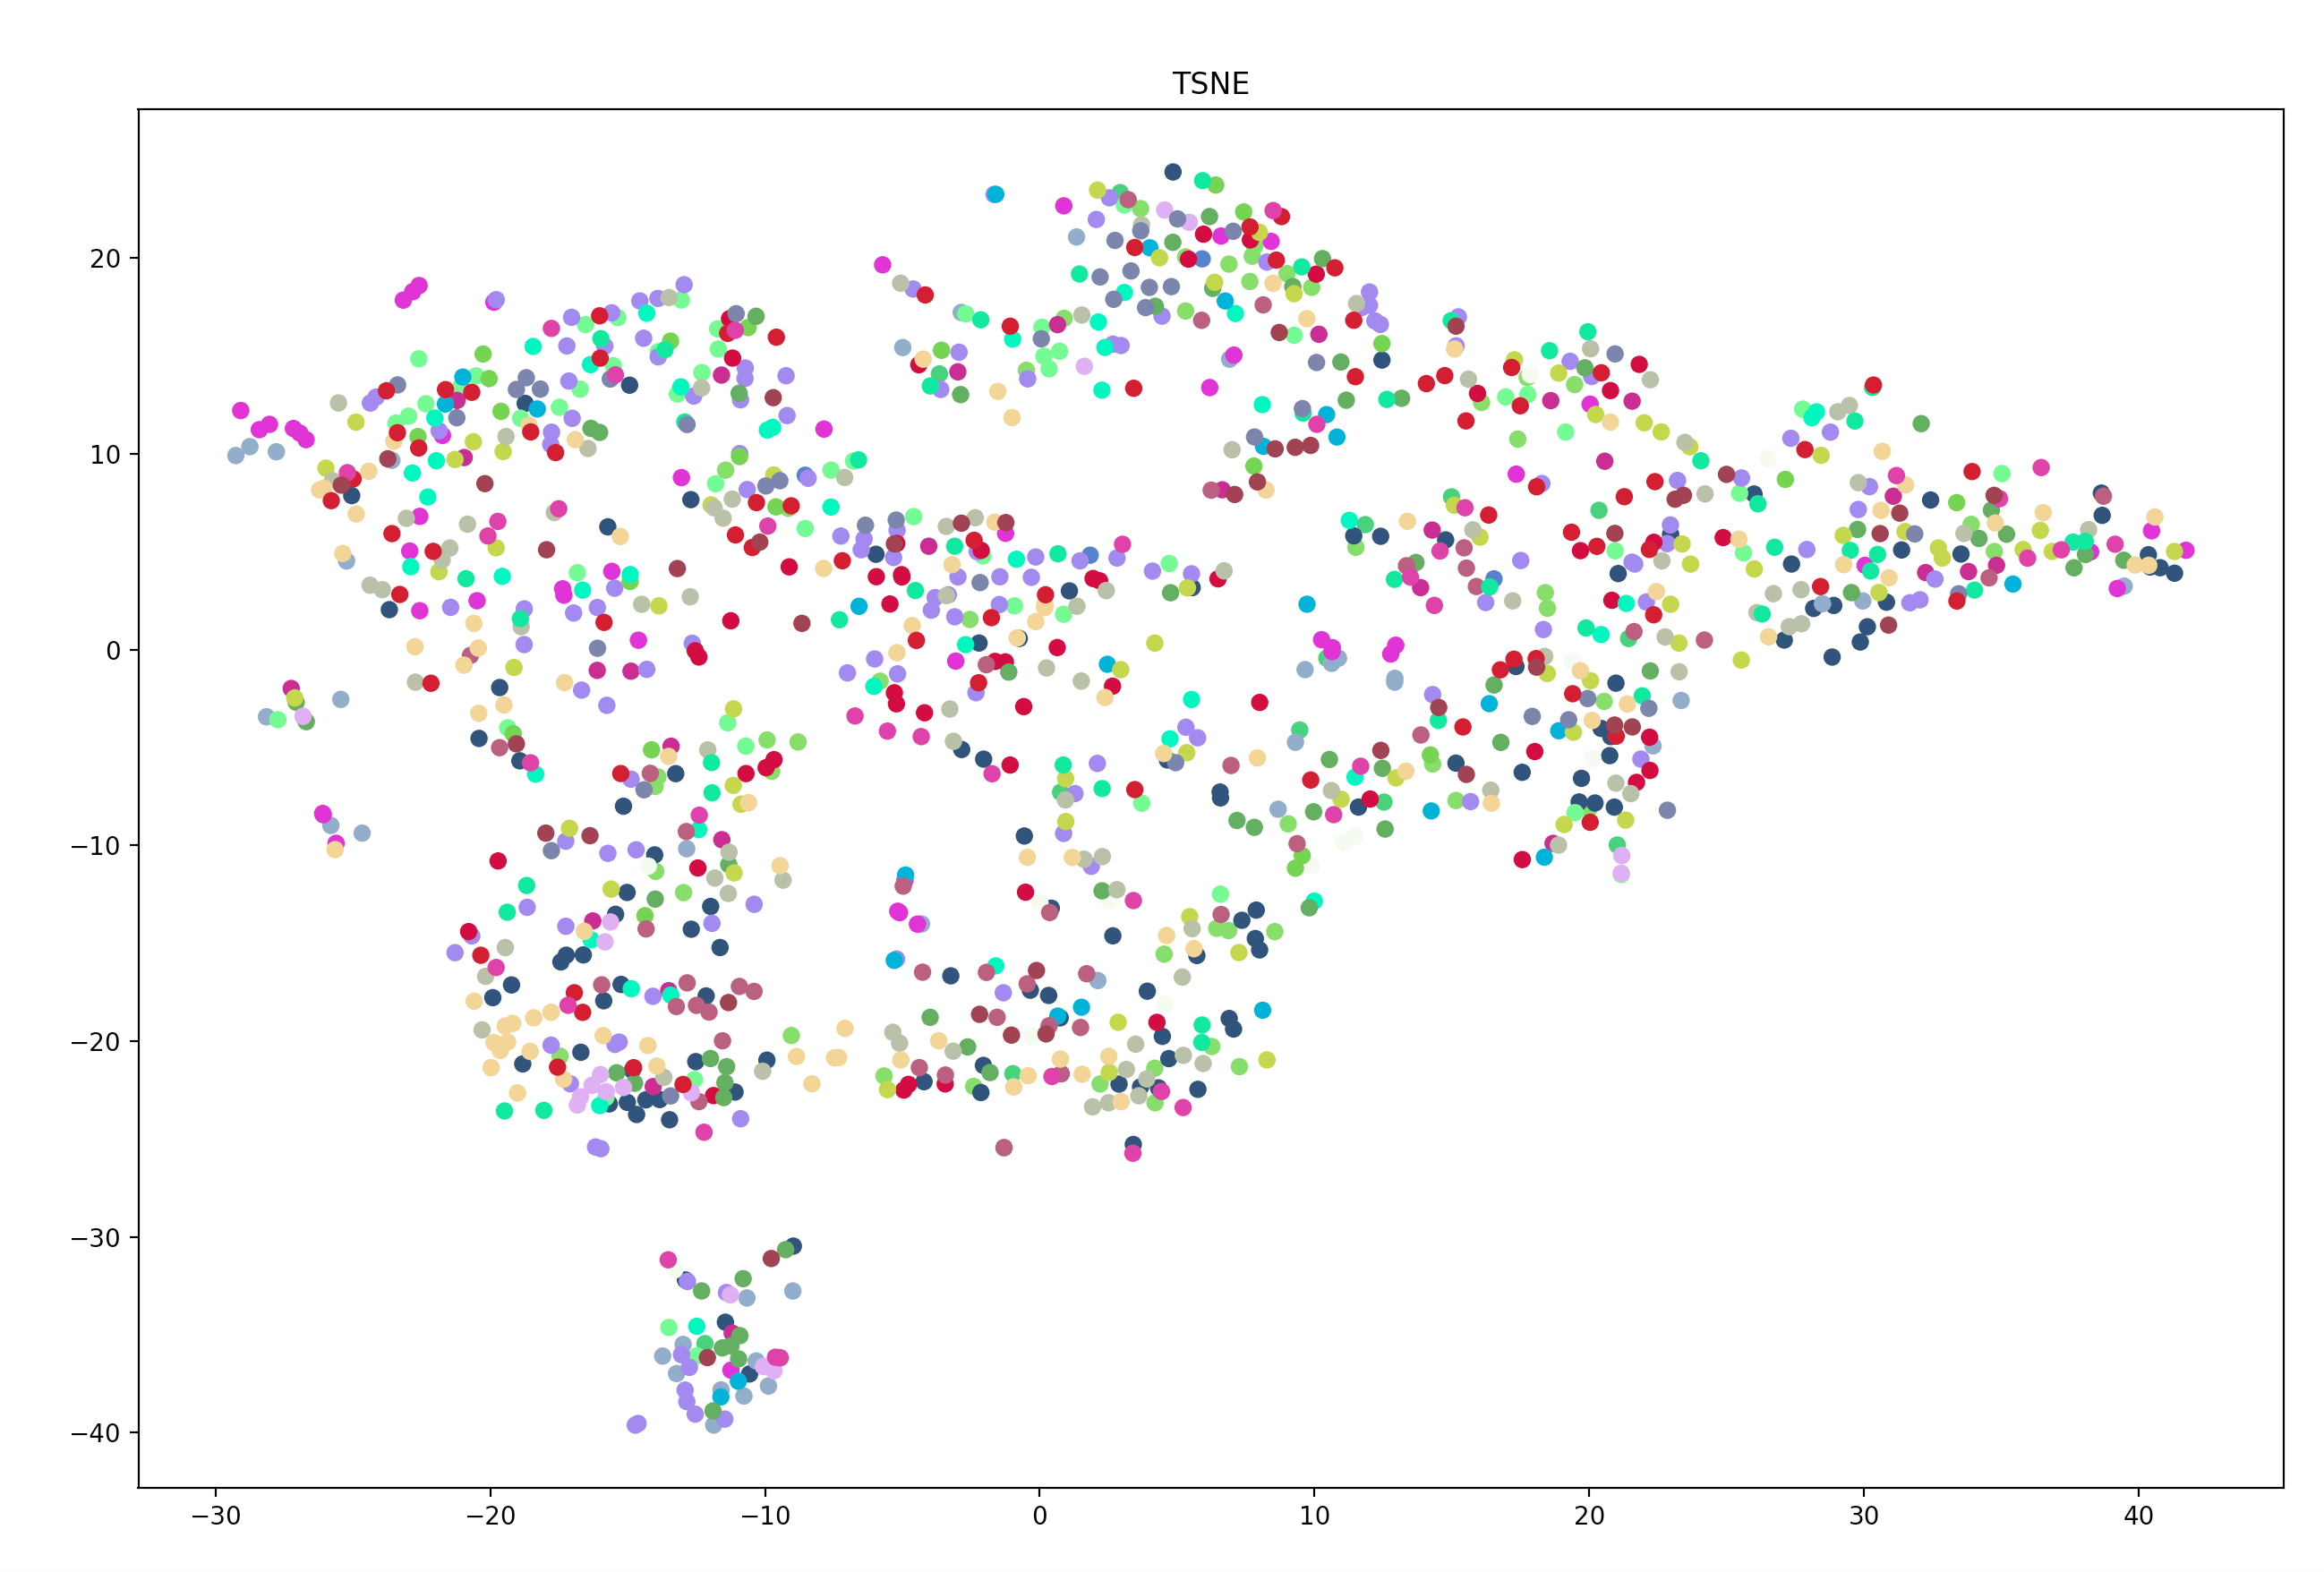
\includegraphics[width=0.9\textwidth]{./images/tsneAfterChainRemoved(60Percent).png}
%   \caption{t-SNE calculated after the removal of rows with less than 60\% of values that weren't 0. The chain is no longer visible.}
%   \label{figure:tsneAfterChainRemoved(60Percent)}
% \end{figure*}

% \begin{figure*}[h]
%   \centering
%   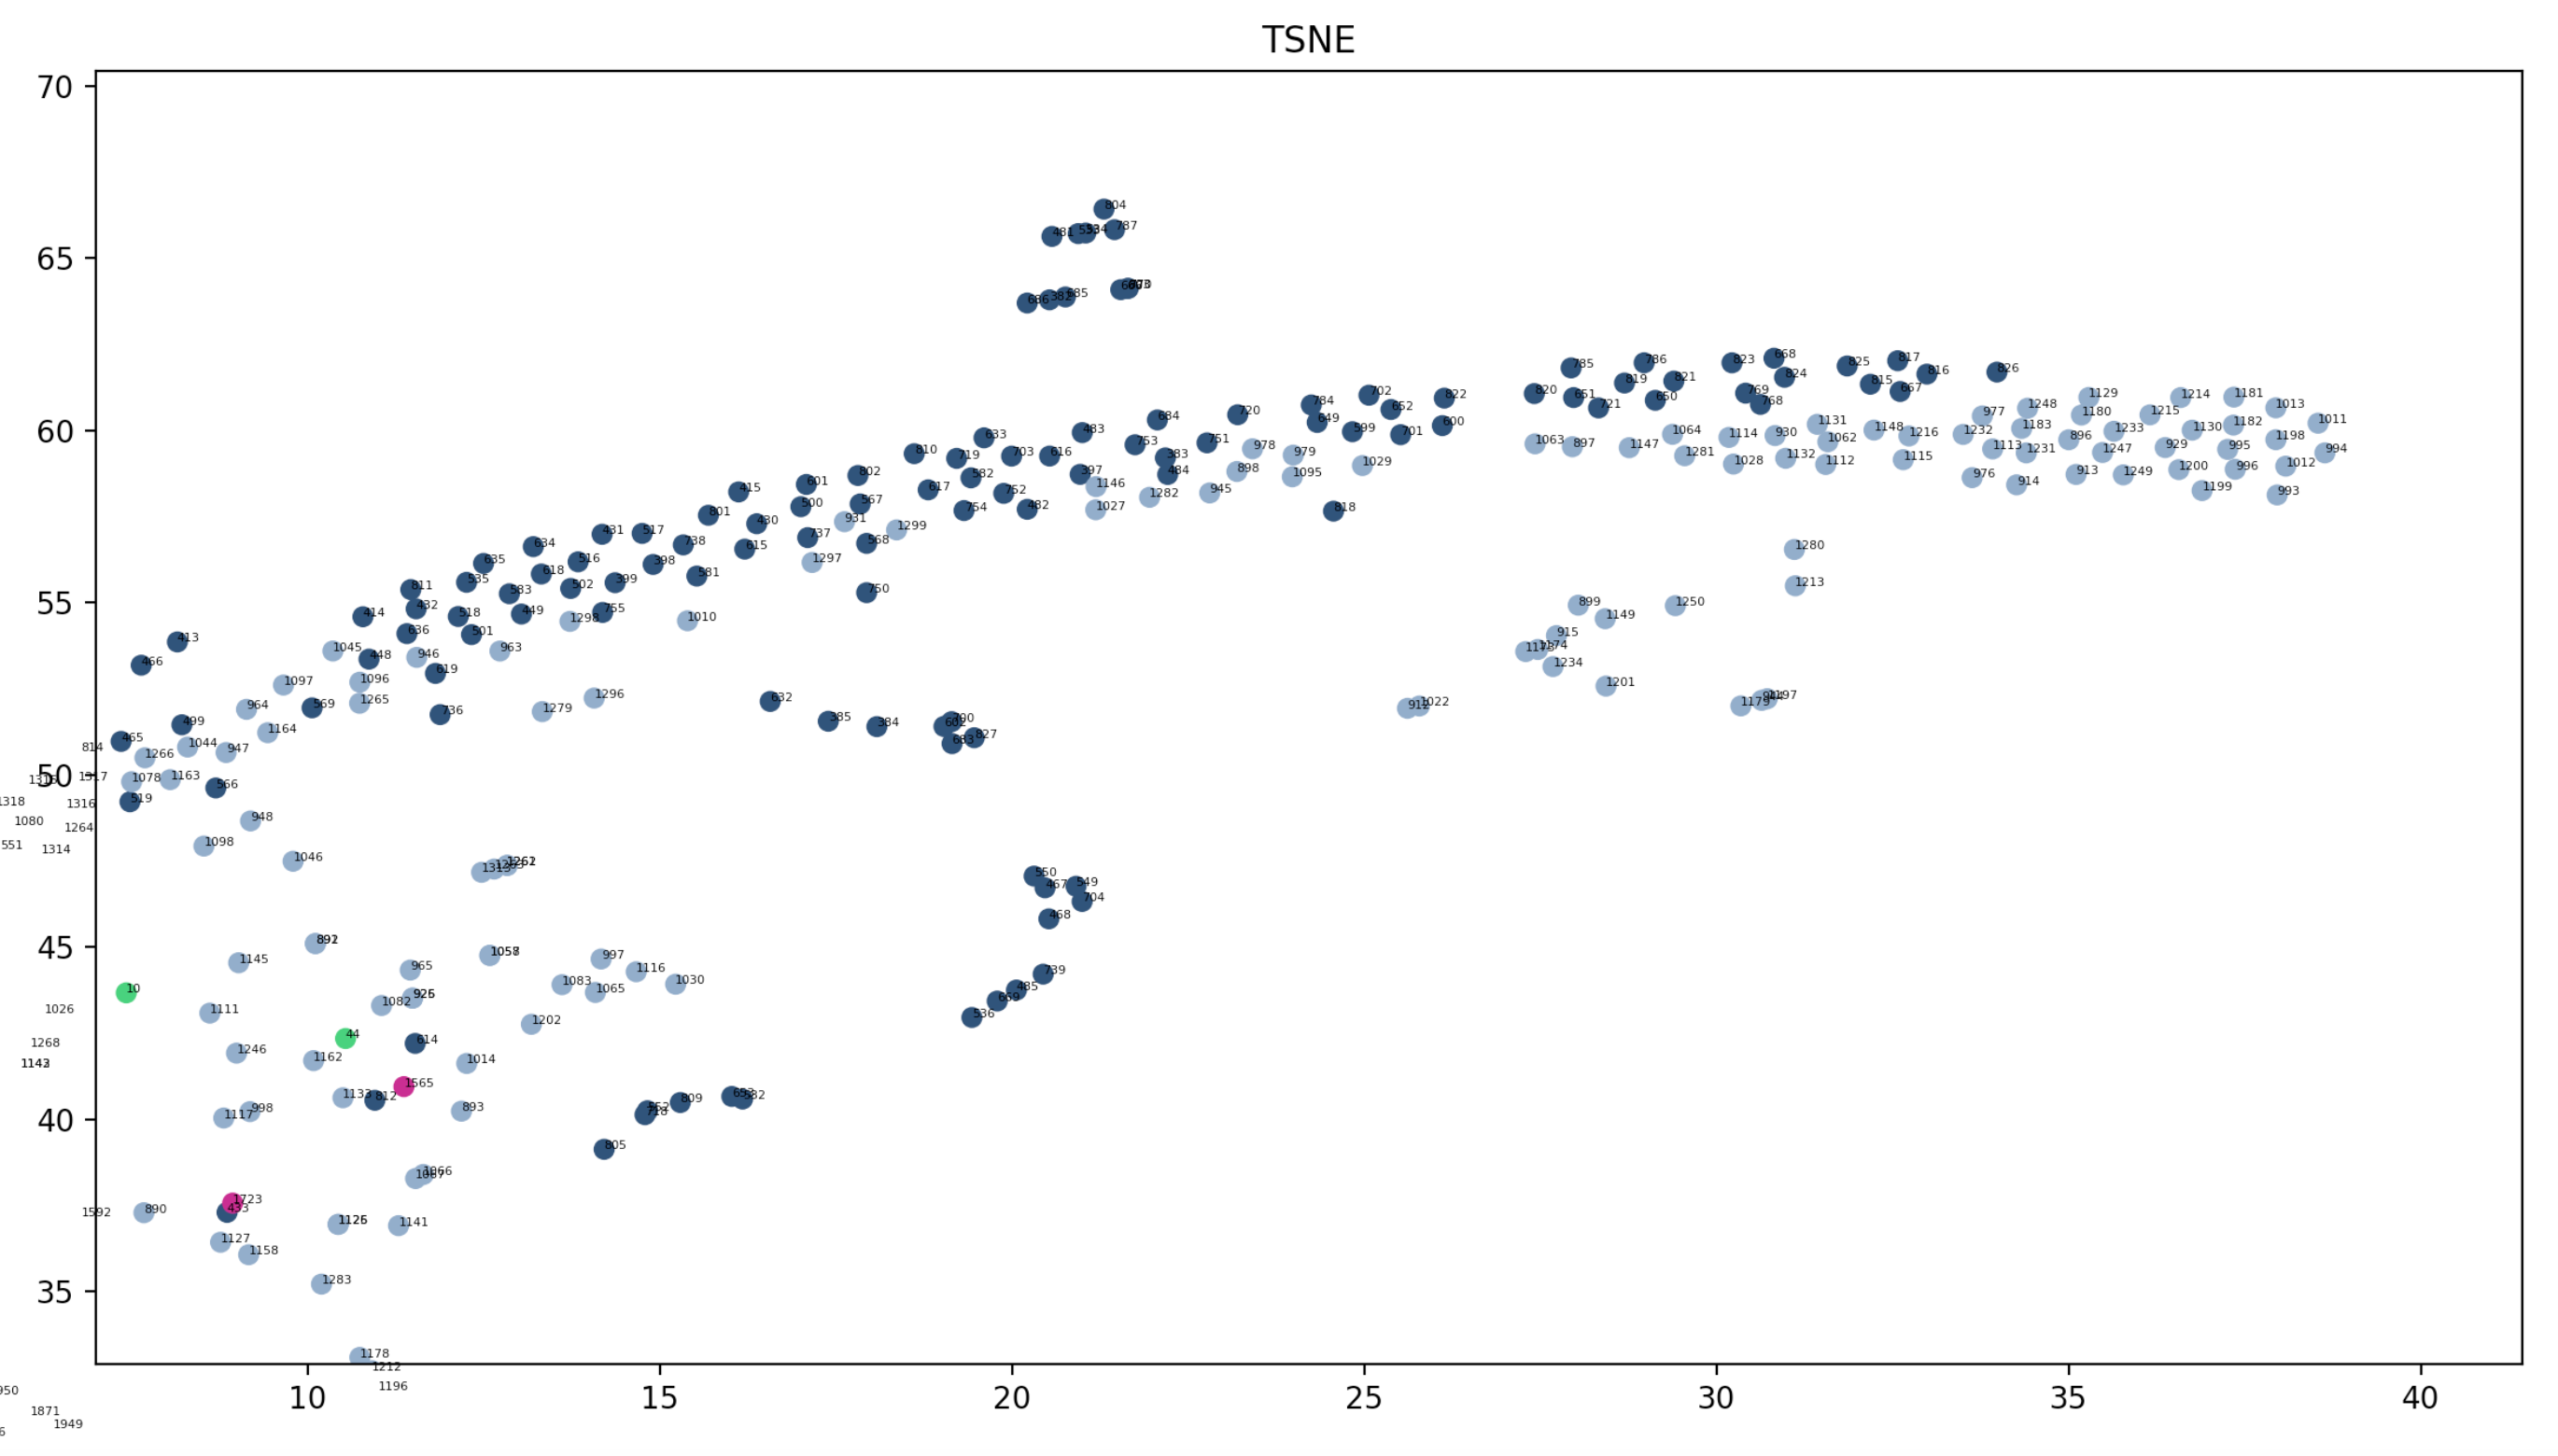
\includegraphics[width=0.9\textwidth]{./images/tsneTestSubjectsColorZoom1.png}
%   \caption{}
%   \label{figure:tsneTestSubjectsColorZoom1}
% \end{figure*}

% \begin{figure*}[h]
%   \centering
%   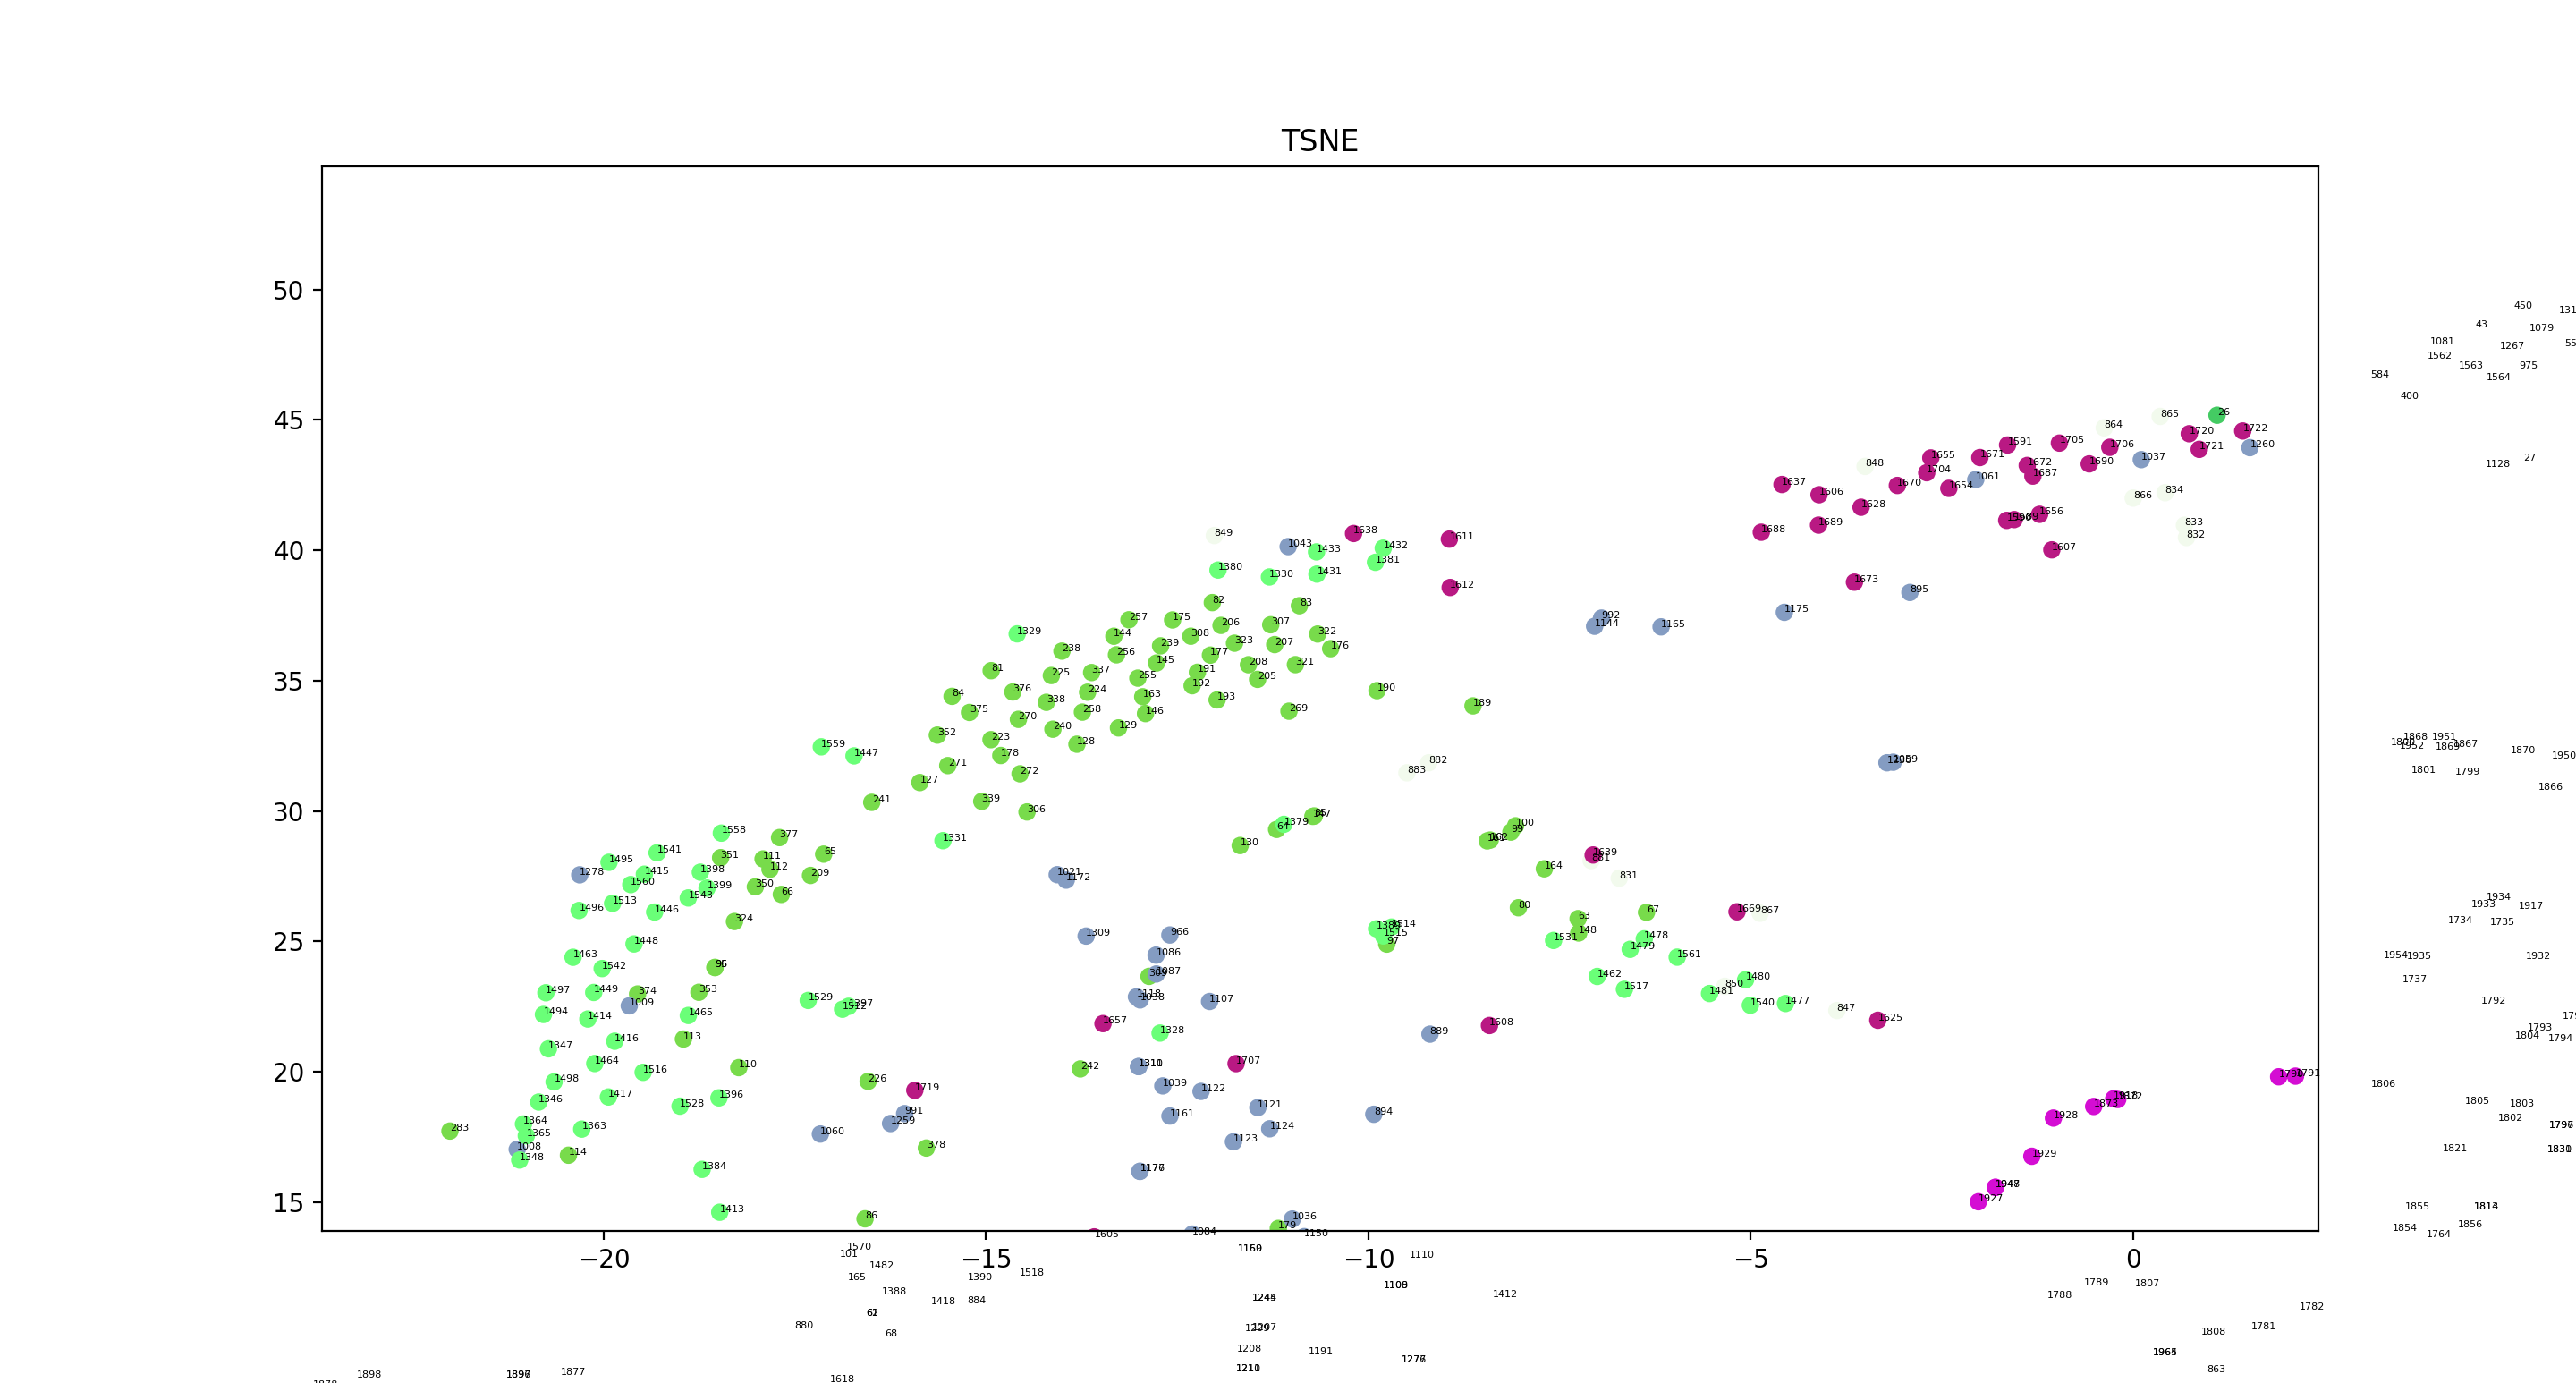
\includegraphics[width=1\textwidth]{./images/tsneTestSubjectsColorZoom2.png}
%   \caption{}
%   \label{figure:tsneTestSubjectsColorZoom2}
% \end{figure*}

% \begin{figure*}[h]
%   \centering
%   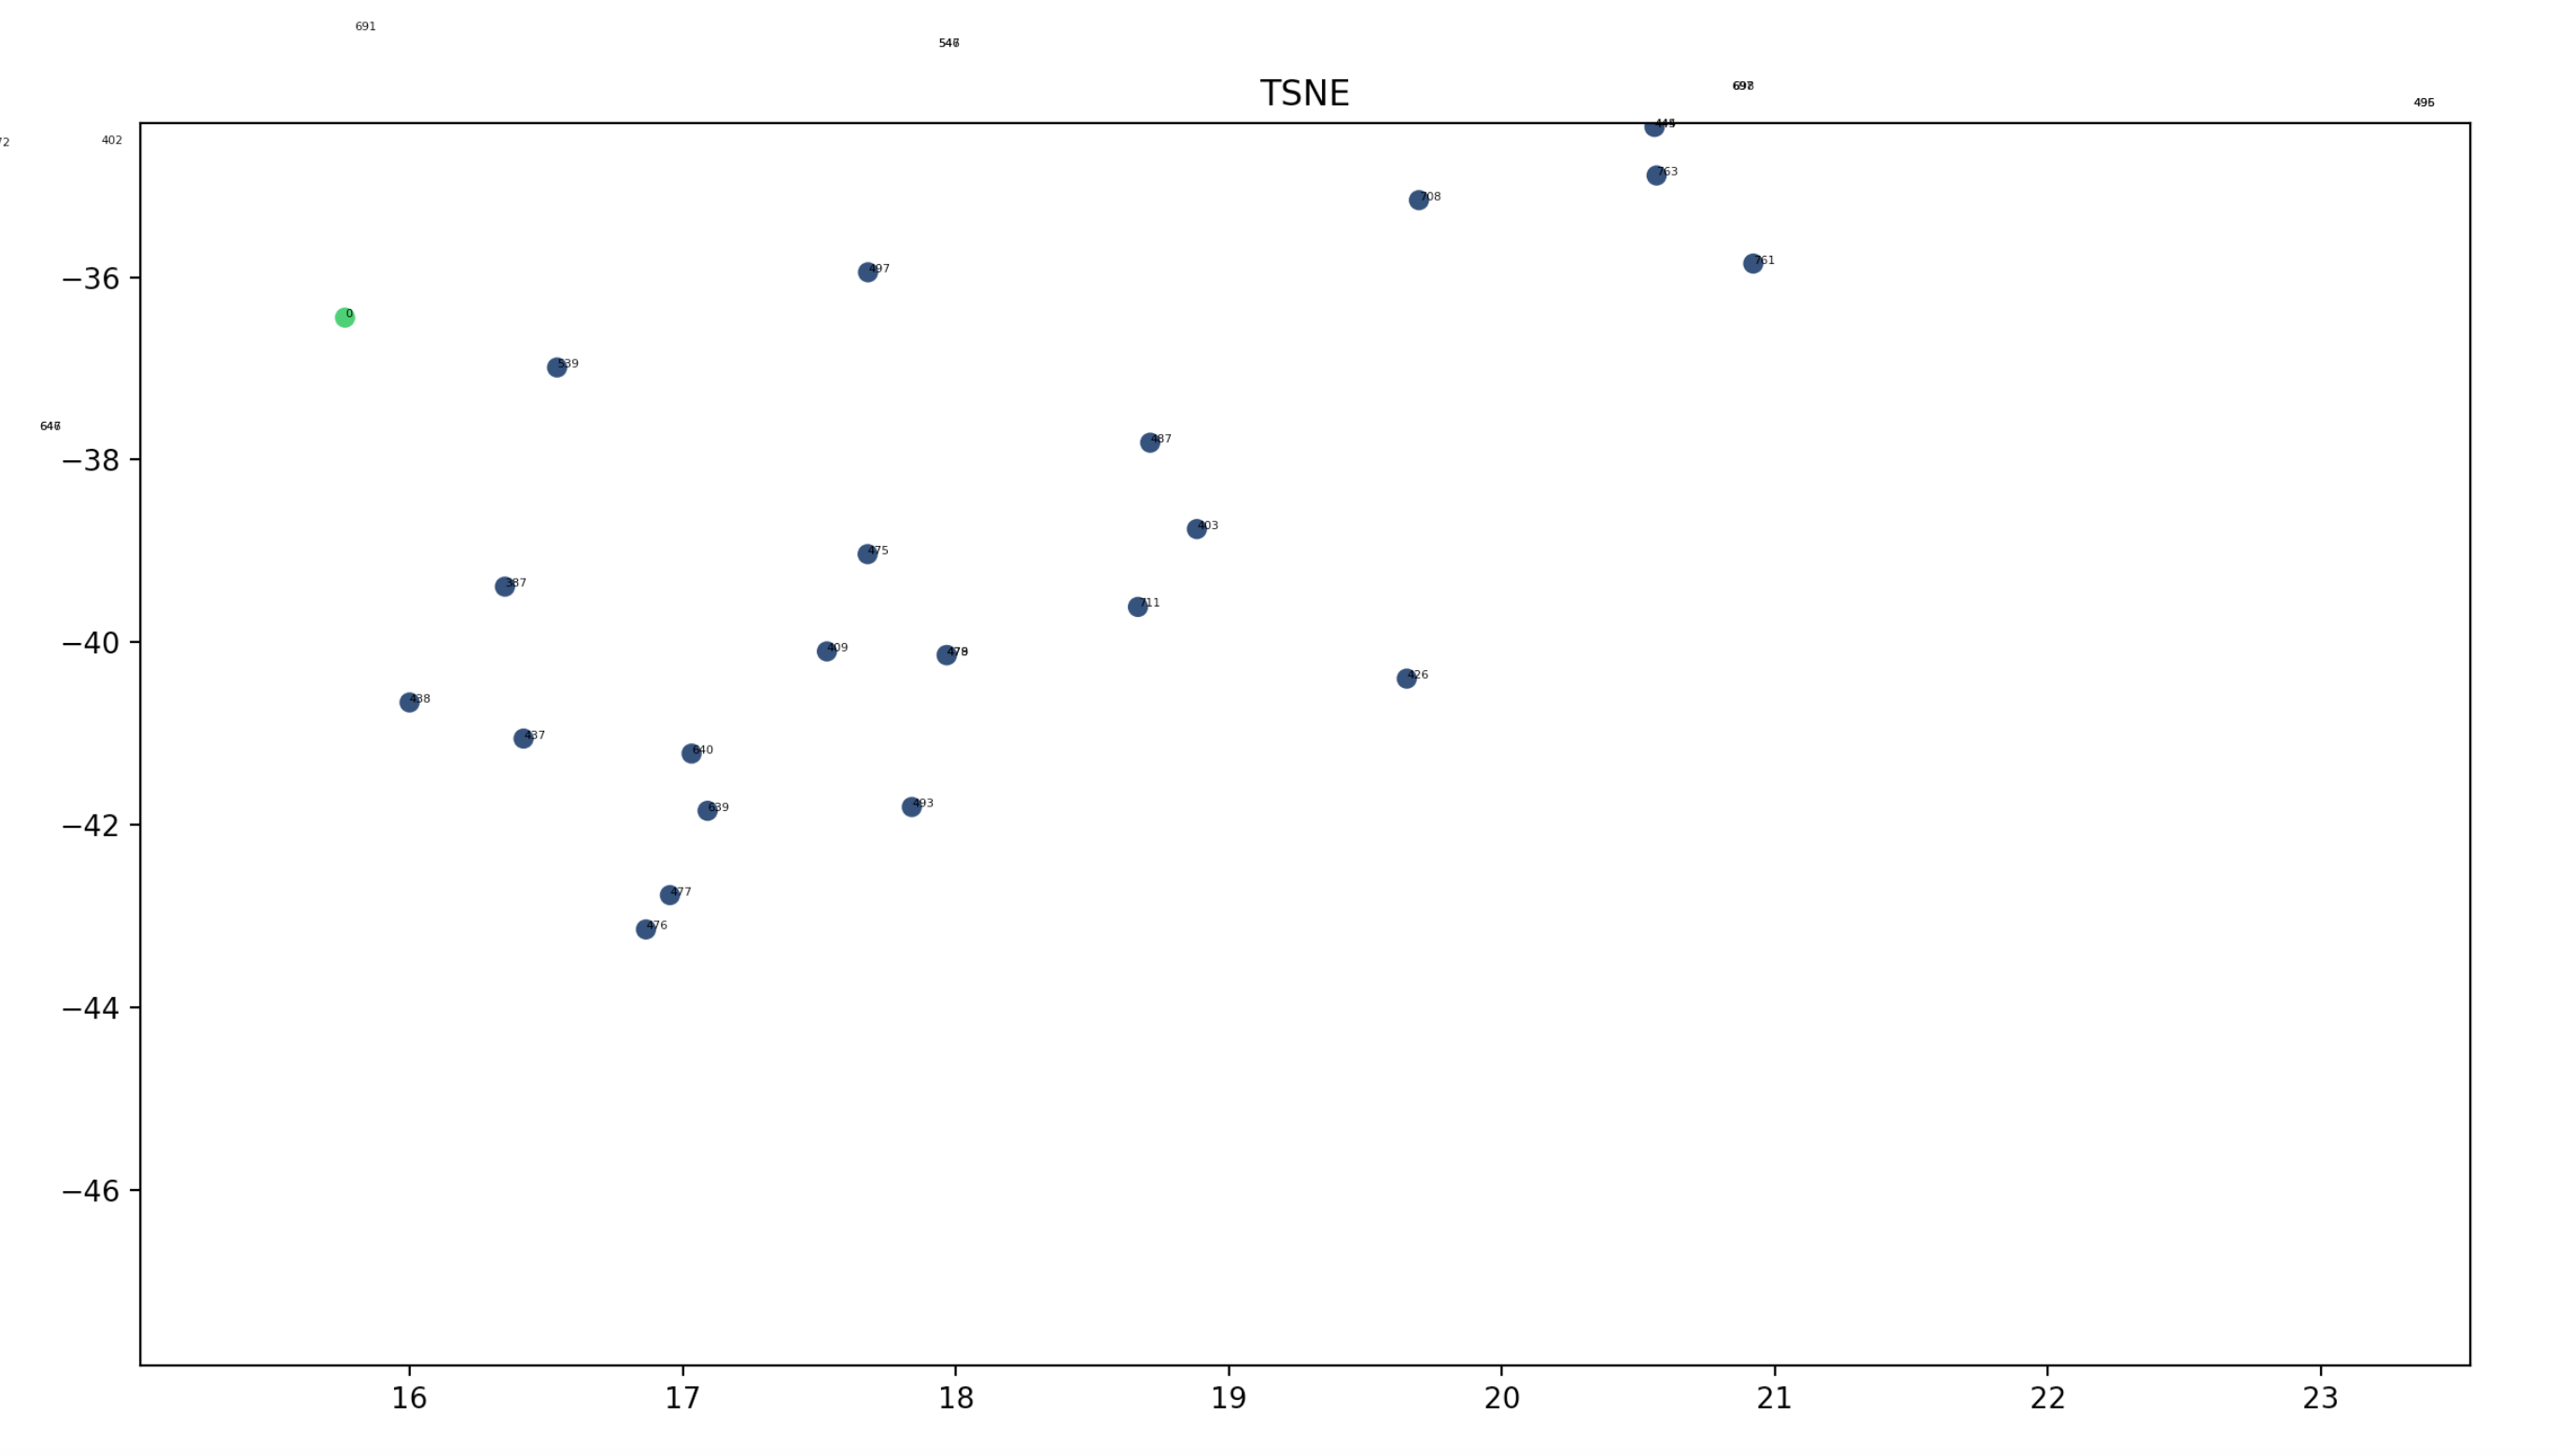
\includegraphics[width=0.9\textwidth]{./images/tsneTestSubjectsColorZoom3.png}
%   \caption{}
%   \label{figure:tsneTestSubjectsColorZoom3}
% \end{figure*}



% Each unique feature only requires one column, and it therefore reduces the number of columns by 

